\documentclass[11pt,a4paper]{article}
\usepackage[utf8]{inputenc}
\usepackage{amsmath}
\usepackage{amsfonts}
\usepackage{dsfont}
\usepackage{amssymb}
\usepackage{array}
\usepackage{latexsym}
\usepackage{textcomp}
\usepackage{graphicx}
\usepackage{fullpage}
\usepackage{float} 
\usepackage{caption}
\usepackage{xcolor}

\title{Optimal Shape Design of Wave-Maker}

\date{}

\begin{document}

\begin{minipage}{15cm}
	\begin{minipage}{7cm}
		ECOLE POLYTECHNIQUE \\
		PROMOTION 2011 \\ 
		GOIX Robin
	\end{minipage}
	\vspace{5\baselineskip}
	\maketitle
	\center\makebox[15cm]{\textbf\dotfill}
	\vspace{1\baselineskip}
	\center{\textbf{NON CONFIDENTIEL}}
	\vspace{6\baselineskip}
	\begin{flushleft}
		\underline{Option:} Mathématiques appliquées
		\vspace{.4\baselineskip}\\
		\underline{Champ de l'option:} Analyse numérique
		\vspace{.4\baselineskip}\\
		\underline{Directeur de l'option:} Grégoire ALLAIRE
		\vspace{.4\baselineskip}\\
		\underline{Directeur de stage:} Enrique ZUAZUA
		\vspace{.4\baselineskip}\\
		\underline{Dates du stage:} 	$\mbox{1}^{\mbox{er}}$ avril 2014 - 30 juin 2014
		\vspace{.4\baselineskip}\\
		\underline{Nom et adresse de l'organisme:}\\
		Basque Center for Applied Mathematics\\
		Alameda Mazarredo, 14\\
		48009 Bilbao, Vizcaya\\
		Espagne
	\end{flushleft}
\end{minipage}

\pagebreak

\tableofcontents
\addcontentsline{toc}{section}{Introduction}

\pagebreak

\section*{Abstract}



\section*{Introduction}
	The aim of this report is to provide a mathematical and computational framework for the problem of water wave generation. Our interest is in modelling the generation of wave by an underwater moving object, to develop a computational framework for this problem and then to use it in order to optimize the shape and trajectory of the underwater moving object.
		
	\pagebreak
		
\section{Derivation of the Peregrine System}\label{Part1}
	The first step is to derive an appropriate model to represent our problem. We aim at modelling the creation and propagation of breaking waves to surf, which occurs near the shore where the seabed rises. We will therefore make some assumptions so as to find an accurate model as simple as possible. We will consider water as an incompressible and inviscid fluid to derive the physical model we will use, using the work of \cite{DM2013} in the case of tsunamis generated by a moving bottom disturbance.
	
	As illustrated in Figure \ref{Coordinates}, we consider $(\tilde{x},\tilde{y},\tilde{z})$ a Cartesian coordinate system, with $\tilde{z}$ measuring upwards from the still water level. We call $\tilde{\eta}(\tilde{x},\tilde{y},\tilde{t})$ the height of the free surface at a time $\tilde{t}$, and $\tilde{h}(\tilde{x},\tilde{y},\tilde{t}) = \tilde{D}(\tilde{x},\tilde{y}) + \tilde{\zeta}(\tilde{x},\tilde{y}, \tilde{t})$ the seabed profile, which is assumed to be the sum of a time-independent part $\tilde{D}$ - the seabed -, and a time-dependant part $\tilde{\zeta}$ - the underwater moving object.
	\begin{figure}[h]
		\centering
		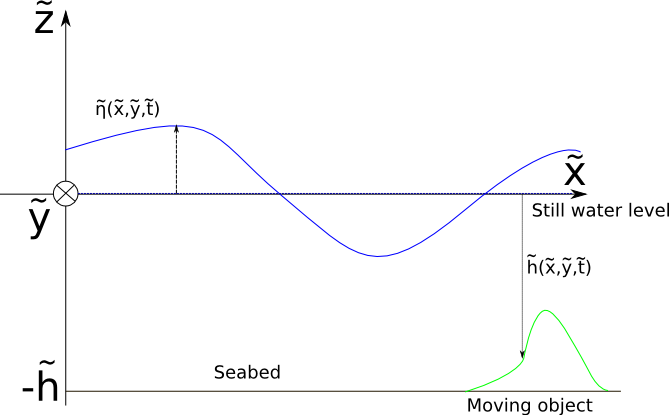
\includegraphics[height=6cm]{CartesianCoordinates.png}
		\caption{Reference}
		\label{Coordinates}
	\end{figure}
			
	Denoting $\mathbf{\hat{u}} = (\tilde{u},\tilde{v}, \tilde{w})$ the fluid velocity, $\hat{P}$ the pressure field, $\rho$ the density and $\mathbf{g} = (0,0,g)$ the gravity, the Euler equations are written: 
	\begin{align}
		\displaystyle \mathbf{\hat{u}}_{\tilde{t}} + (\mathbf{\hat{u}} \cdot \tilde{\nabla}) \mathbf{\hat{u}} + \frac{1}{\rho} \tilde{\nabla}\tilde{P} &=  -\mathbf{g} \label{Euler1} \\
		\tilde{\nabla} \cdot \mathbf{\hat{u}} & = 0 \\
		\tilde{\nabla} \times \mathbf{\hat{u}} & = 0 \label{Euler3}
	\end{align}
	The kinematic boundary condition at the free surface expresses the equality between the vertical velocity and the total derivative of $\tilde{\eta}$, whereas the kinematic boundary condition at the bottom expresses the equality between the vertical velocity and the total derivative of $\tilde{h}$:
	\begin{align}
		\frac{\mathrm{d}}{\mathrm{d}\tilde{t}} \tilde{\eta}(\tilde{x},\tilde{y},\tilde{t}) & = \tilde{w}(\tilde{x},\tilde{y},\tilde{\eta}) \label{BC1} \\
		-\frac{\mathrm{d}}{\mathrm{d}\tilde{t}} \tilde{h}(\tilde{x},\tilde{y},\tilde{t}) & = \tilde{w}(\tilde{x},\tilde{y},-\tilde{h}) \label{BC2}
	\end{align}
	At the free surface $\tilde{z} = \tilde{\eta}(\tilde{x},\tilde{y},\tilde{t})$,	the fluid is also assumed to satisfy the dynamic boundary condition $\tilde{P}(\tilde{x},\tilde{y},\tilde{t}) = \tilde{P}_0(\tilde{x},\tilde{y})$.
			
	Considering a characteristic water depth $h_0$ and the corresponding 	characteristic velocity $c_0 = \sqrt{g h_0}$, a typical wavelength $\lambda_0$ and a typical wave height $a_0$, we use the following scaled variables: 
	\begin{equation*}
		x = \frac{\tilde{x}}{\lambda_0},\: 
		y = \frac{\tilde{y}}{\lambda_0}, \:
		z = \frac{\tilde{z}}{h_0}, \: 
		t = \frac{c_0}{\lambda_0}\tilde{t}
	\end{equation*}
	\begin{equation*}
		u = \frac{h_0}{a_0 c_0} \tilde{u},\:
		v = \dfrac{h_0}{a_0 c_0} \tilde{v},\:
		w = \dfrac{\lambda_0}{a_0 c_0} \tilde{w},\: 
		\eta = \dfrac{\tilde{\eta}}{a_0},\: 
		h = \dfrac{\tilde{h}}{h_0},\:
		D = \dfrac{\tilde{D}}{h_0}, \:
		\zeta = \dfrac{\tilde{\zeta}}{a_0},\:
		P = \dfrac{\tilde{P}}{\rho c_0^2}				
	\end{equation*}
	We separate the vertical and horizontal velocity, such as $\mathbf{u} = (u,v)$ and $\nabla = (\partial_x,\partial_y)$, and we consider $\epsilon = a_0 / h_0$ and $\sigma = h_0 / \lambda_0$ to be small. The dimensionless form of the equations \eqref{Euler1} - \eqref{Euler3} are therefore given by: 
	\begin{align}
		\epsilon \mathbf{u}_t + \epsilon^2((\mathbf{u} \cdot \nabla) \mathbf{u} + w \mathbf{u}_z) + \nabla P & = 0 \label{MConsxy}\\
		\epsilon \sigma^2 w_t + \epsilon^2 \sigma^2 ((\mathbf{u} \cdot \nabla w) + w w_z) + P_z & = -1 \label{MConsz}\\
		\nabla \cdot \mathbf{u} + w_z & =  0 \label{MassCons}\\
		u_y-v_x & = 0 \label{Irrxy}\\
		\mathbf{u}_z - \sigma^2 \nabla w & = 0 \label{Irrz}
	\end{align}
	and the dimensionless form of the boundary conditions \eqref{BC1} - \eqref{BC2} are: 
	\begin{align}
		\eta_t + \epsilon (\mathbf{u} \cdot \nabla \eta ) & = w & \mathrm{on} \: z =\epsilon \eta \label{BCH}\\
		- \zeta_t - \mathbf{u} \cdot \nabla h & = w & \mathrm{on} \:  z = -h
		\label{BCB}
	\end{align}
	where $h = D + \epsilon \zeta $.
			
	Integrating equation \eqref{MassCons} with respect to $z$ from $-h$ to $z$, and using \eqref{BCB} we have: 
	\begin{equation}
		w = -\mathbf{u} \cdot \nabla h - \int^z_{-h} \nabla \cdot \mathbf{u} - \zeta_t 
		\label{Eq1}
	\end{equation}
	After integration of equation \eqref{Irrz} and using \eqref{Eq1}, we observe 
	\begin{equation}
		\mathbf{u} = \mathbf{u}_b + O(\sigma^2) \label{ApproxVelocity}
	\end{equation}
	where $\mathbf{u}_b$ is the horizontal velocity of the fluid at the bottom $z=-h$. Substitution of \eqref{Eq1} into the irrotationality condition \eqref{Irrz}, and using \eqref{ApproxVelocity}, yields:
	\begin{equation}
		\mathbf{u}_z = -\sigma^2\nabla(\nabla \cdot (h \mathbf{u}_b)) - \sigma^2 z \nabla(\nabla \cdot \mathbf{u}_b) - \sigma^2 \nabla \zeta_t + O(\sigma^4) 
		\label{Eq:u_z}
	\end{equation}
	Integration of \eqref{Eq:u_z} with respect to $z$ from $-h$ to $z$ gives
	\begin{equation}
		\mathbf{u} = \mathbf{u}_b - \sigma^2(z+h)\nabla (\nabla \cdot (h \mathbf{u}_b)) - \sigma^2 \frac{z^2-h^2}{2}\nabla ( \nabla \cdot \mathbf{u}_b) - \sigma^2(z+h)\nabla \zeta_t + O(\sigma^4) \label{ApproxVelocity2}
	\end{equation}
	We note than \eqref{ApproxVelocity} and \eqref{Eq1} lead to: 
	\begin{equation}
		w = - \nabla \cdot (h \mathbf{u}_b) - z \nabla \cdot \mathbf{u}_b - \zeta_t + O(\sigma^2)
	\end{equation}
	and then:
	\begin{equation}
		w_t = - \nabla \cdot (h \mathbf{u}_b)_t - z \nabla \cdot (\mathbf{u}_b)_t - \zeta_{tt} + O(\sigma^2) \label{Eq:2} 
	\end{equation}
	Assuming that $P = 0$ at $z = \epsilon\eta$, integrating \eqref{MConsz} with respect to $z$ from $z$ to $\epsilon\eta$, and using \eqref{Eq:2} we obtain
	\begin{equation}
		P = \epsilon \sigma^2(z\nabla \cdot (h \mathbf{u}_b)_t + \frac{z^2}{2} \nabla \cdot (\mathbf{u}_b)_t) + \epsilon \sigma^2z \zeta_{tt} + \epsilon \eta - z + O(\epsilon\sigma^4, \epsilon^2 \sigma^2) \label{Pressure}
	\end{equation}
	Using equations \eqref{MConsxy} and \eqref{ApproxVelocity2}, for $z = -h$, and considering the fact that $h_t = O(\epsilon)$, we have
	\begin{equation}
		(\mathbf{u}_b)_t + \nabla \eta + \epsilon (\mathbf{u}_b \cdot \nabla)\mathbf{u}_b - \sigma^2 h \nabla (\nabla \cdot (h (\mathbf{u}_b)_t)) + \sigma^2 \frac{h^2}{2} \nabla (\nabla \cdot (\mathbf{u}_b)_t) - \sigma^2 h \nabla \zeta_{tt} = O(\sigma^4, \epsilon \sigma ^2) \label{Eq:3}
	\end{equation}
	Integration of the conservation of mass \eqref{MassCons} with respect to $z$ from $-h$ to $\epsilon\eta$ yields
	\begin{equation}
		w(\epsilon\eta) - w(-h) = - \int^{\epsilon\eta}_{-h} \! \nabla \cdot \mathbf{u} \; \mathrm{dz}
	\end{equation}
	and thus, adding the boundary conditions \eqref{BCB} and \eqref{BCH} we have
	\begin{equation}
		\eta_t + \nabla \cdot \int^{\epsilon\eta}_{-h}\ \mathbf{u} \; \mathrm{dz} 
		\label{BoundaryEq}
	\end{equation}
			
	Denote the depth-average horizontal velocity of the fluid by 
	\begin{equation}
		\bar{\mathbf{u}} = \frac{1}{h+\epsilon \eta} \int^{\epsilon\eta}_{-h}\! \mathbf{u} \; \mathrm{dz}
		\label{AverageVelocity}
	\end{equation}
	then \eqref{BoundaryEq} becomes 
	\begin{equation}
		\eta_t + \zeta_t + \nabla \cdot [(h + \epsilon \zeta) \bar{\mathbf{u}}] = 0 
		\label{Eq:Sys2}
	\end{equation}
	Using the depth-average velocity \eqref{AverageVelocity} in \eqref{ApproxVelocity2} we obtain: 
	\begin{equation}
		\mathbf{u}_b = \bar{\mathbf{u}} + \sigma^2\frac{h}{2} \nabla (\nabla \cdot (h \bar{\mathbf{u}}) - \sigma^2 \frac{h^2}{3} \nabla (\nabla \cdot \bar{\mathbf{u}}) + \sigma^2 \frac{h}{2} \nabla \zeta_t + O(\sigma^4, \epsilon \sigma^2)
		\label{AverageVelocity2}
	\end{equation}
	and thus, the equation \eqref{Eq:3} gives: 
	\begin{equation}
		\bar{\mathbf{u}}_t + \nabla \eta + \epsilon(\bar{\mathbf{u}} \cdot \nabla) \bar{\mathbf{u}} - \sigma^2 \frac{h}{2} \nabla ( \nabla \cdot (h\bar{\mathbf{u}}_t)) + \sigma^2 \frac{h^2}{6}\nabla ( \nabla \cdot \bar{\mathbf{u}}_t) - \sigma^2\frac{h}{2}\nabla \zeta_{tt} = O(\epsilon \sigma^2, \sigma^4) 
		\label{Eq:Sys1}
	\end{equation}
			
	To reduce the amount of notation, the depth-average velocity will subsequently be denoted $\mathbf{u}$. With equations \eqref{Eq:Sys1} and \eqref{Eq:Sys2}, we obtain the Boussinesq system of equations similar to \cite{Peregrine}.
	\begin{center}
		$\left\lbrace
			\begin{array}{rll}
				\displaystyle \mathbf{u}_t + \nabla \eta + \epsilon (\mathbf{u} \cdot \nabla)\mathbf{u} - \sigma^2\frac{h}{2}\nabla (\nabla \cdot (h \mathbf{u}_t)) + \sigma^2 \frac{h^2}{6}\nabla (\nabla \cdot \mathbf{u}_t) - \sigma^2\frac{h}{2}\nabla \zeta_{tt}  & = & \displaystyle O(\epsilon \sigma^2, \sigma^4) \\
				\displaystyle \eta_t+\zeta_t + \nabla \cdot [(h+\epsilon\eta)\mathbf{u}] & = & 0
			\end{array}
		\right.$
	\end{center}
			
	We can immediately notice that this system is very close to the classical shallow water equations (\eqref{SWE1}, \eqref{SWE2}), and contains only three added termes of order $\sigma^2$:
	\begin{align}
		\mathbf{u}_t + \nabla\eta + \epsilon (\mathbf{u} \cdot \nabla) \mathbf{u} &= 0 \label{SWE1}\\
		\eta_t + \zeta_t + \nabla \cdot [(h+\epsilon \eta) \mathbf{u}] &= 0 \label{SWE2}
	\end{align}	
			
	\pagebreak
			
\section{Numerical solver for the Peregrine system}	
	In this section, we will establish a numerical scheme to be able to solve the previous system with a finite element method. This scheme will be the foundation of our forward model to run the optimization process on the object's shape.
	
\subsection{Weak Formulation of the Peregrine system}
	We consider the Peregrine system derived in the previous section: 
	\begin{align}
		\mathbf{u}_t + \nabla \eta + \epsilon (\mathbf{u} \cdot \nabla)\mathbf{u} - \sigma^2\frac{h}{2}\nabla (\nabla \cdot (h \mathbf{u}_t)) + \sigma^2 \frac{h^2}{6}\nabla (\nabla \cdot \mathbf{u}_t) - \sigma^2\frac{h}{2}\nabla \zeta_{tt}  &= O(\epsilon \sigma^2, \sigma^4) \label{Peregrine1}\\
		\eta_t+\zeta_t + \nabla \cdot [(h+\epsilon\eta)\mathbf{u}] &= 0 \label{Peregrine2}
	\end{align}	
	The well-posedness of Boussinesq systems (including the Peregrine system) as been studied in \cite{QuinteroMunoz}, but do not mention any boundary conditions. 	Considering the fluid to be in a pool, we impose slip boundary conditions for the velocity on $\partial \Omega$, and introduce the space $\mathbb{V} = \left\lbrace \mathbf{w} \in \mathbb{H}^1(\Omega)^2, \mathbf{w} \cdot \mathbf{n} = 0 \: \mathrm{on} \: \partial \Omega \right\rbrace $, where $\mathbf{n}$ represent the normal to the boundary. In that case and as all the boundary termes including $\eta$ and coming from the divergence theorem are of the form $\eta (\mathbf{u} \cdot \mathbf{n})$, we can avoid to impose boundary conditions on the height $\eta$, as done in \cite{HanertLegatDeleersnijder} and \cite{DawsonMartinez} for the case of the shallow water equations. Let $(\mathbf{v},\xi) \in \mathbb{V} \times \mathbb{H}^1(\Omega)$, then multiplying \eqref{Peregrine1} by $\mathbf{v}$ and \eqref{Peregrine2} by $\xi$ and integrating over the domain $\Omega$, we obtain:   
	\begin{equation}
		\begin{split}
			&\int_{\Omega} \! \mathbf{u}_t \cdot \mathbf{v} \: \mathrm{dx} + \int_{\Omega} \! \nabla \eta \cdot \mathbf{v} \: \mathrm{dx} + \epsilon \! \int_{\Omega} \! (\mathbf{u} \cdot \nabla ) \mathbf{u} \cdot \mathbf{v} \: \mathrm{dx} - \sigma^2 \! \int_{\Omega} \! \frac{D + \epsilon \zeta}{2} \nabla (\nabla \cdot ((D + \epsilon \zeta) \mathbf{u}_t)) \cdot \mathbf{v} \: \mathrm{dx} \\
			&\qquad + \sigma^2 \! \int_{\Omega} \! \frac{(D + \epsilon \zeta)^2}{6} \nabla (\nabla \cdot \mathbf{u}_t) \cdot \mathbf{v} \: \mathrm{dx} - \sigma^2 \! \int_{\Omega} \! \frac{D + \epsilon \zeta}{2} \nabla \zeta_{tt} \cdot \mathbf{v} \: \mathrm{dx} = 0\\
			&\int_{\Omega}\! \eta_t \; \xi \: \mathrm{dx} +\int_{\Omega}\! \zeta_t \; \xi \: \mathrm{dx} +\int_{\Omega}\! \nabla \cdot [(D + \epsilon \zeta+\epsilon\eta) \mathbf{u}] \; \xi \: \mathrm{dx} = 0
		\end{split}
		\label{PeregrineWeakForm1}
	\end{equation}
	Using divergence theorem and the fact that $\mathbf{v} \cdot \mathbf{n}$ and $\mathbf{u} \cdot \mathbf{n}$ vanish on the boundaries, we get: 
	\begin{equation}
		\begin{split}
			&\int_{\Omega} \! \mathbf{u}_t \cdot \mathbf{v} \: \mathrm{dx} - \int_{\Omega} \! \eta \; (\nabla \cdot \mathbf{v}) \: \mathrm{dx} + \epsilon \! \int_{\Omega} \! (\mathbf{u} \cdot \nabla ) \mathbf{u} \cdot \mathbf{v} \: \mathrm{dx} + \frac{\sigma^2}{2} \! \int_{\Omega} \!  (\nabla \cdot ((D + \epsilon \zeta) \mathbf{u}_t)) \; (\nabla \cdot ((D + \epsilon \zeta) \mathbf{v}) )\: \mathrm{dx} \\
			&\qquad - \frac{\sigma^2}{6} \! \int_{\Omega} \! (\nabla \cdot \mathbf{u}_t) \; (\nabla  \cdot ((D + \epsilon \zeta)^2  \mathbf{v})) \: \mathrm{dx} + \frac{\sigma^2}{2} \! \int_{\Omega} \!  \zeta_{tt}  \; (\nabla \cdot( (D + \epsilon \zeta) \mathbf{v})) \: \mathrm{dx} = 0\\
			 &\int_{\Omega}\! \eta_t \; \xi \: \mathrm{dx} +\int_{\Omega}\! \zeta_t \; \xi \: \mathrm{dx} -\int_{\Omega}\! \nabla \xi \; \cdot [(D + \epsilon \zeta+\epsilon\eta) \mathbf{u}]  \: \mathrm{dx} = 0
		\end{split} 
	\end{equation}
				
\subsection{Time stepping methods}	
	Considering $\Delta t$ a time-step, the second part is to discretize the time dependency. We will use a $\theta$-method in order to get the possibility to run different time stepping methods. Let $\theta$ be in $[0,1] $ and $f$ be a time-dependent function: 	
	\begin{equation}
		\left\lbrace
			\begin{array}{l}
				\displaystyle \forall n > 0, f^{n+\theta} = (1-\theta)f^{n} + \theta f^{n+1}\\
				\displaystyle \forall n > 0, f_t^n \simeq \frac{f^n - f^{n-1}}{\Delta t} \\
				\displaystyle \forall n > 1, f_{tt}^n \simeq \frac{f^n -2f^{n-1} + f^{n-2}}{\Delta t^2} 
			\end{array}
		\right.
	\end{equation}
	For each time-step, knowing $\mathbf{u}^{n-1}$ and $\eta^{n-1}$, our weak formulation is therefore: Find $(\mathbf{u},\eta) \in \mathbb{V} \times \mathbb{H}^1(\Omega), \forall (\mathbf{v},\xi) \in \mathbb{V} \times \mathbb{H}^1(\Omega)$: 
	\begin{equation}
		\begin{split}
			0 &= \int_{\Omega} \! \frac{\mathbf{u} - \mathbf{u}^{n-1}}{\Delta t} \cdot \mathbf{v} \: \mathrm{dx} - \int_{\Omega} \! \eta \; (\nabla \cdot \mathbf{v}) \: \mathrm{dx} + \epsilon \! \int_{\Omega} \! (\mathbf{u} \cdot \nabla ) \mathbf{u} \cdot \mathbf{v} \: \mathrm{dx} + \frac{\sigma^2}{2} \! \int_{\Omega} \! \zeta_{tt}  \; (\nabla \cdot( (D + \epsilon \zeta) \mathbf{v})) \: \mathrm{dx} \\ 
			&\quad + \frac{\sigma^2}{2} \! \int_{\Omega} \!  (\nabla \cdot ((D + \epsilon \zeta) \frac{\mathbf{u} - \mathbf{u}^{n-1}}{\Delta t})) \; (\nabla \cdot ((D + \epsilon \zeta) \mathbf{v}) )\: \mathrm{dx} \\
			& \quad- \frac{\sigma^2}{6} \! \int_{\Omega} \! (\nabla \cdot \frac{\mathbf{u} - \mathbf{u}^{n-1}}{\Delta t}) \; (\nabla  \cdot ((D + \epsilon \zeta)^2  \mathbf{v})) \: \mathrm{dx} \\
			\displaystyle 0 &= \int_{\Omega}\! \frac{\eta - \eta^{n-1}}{\Delta t} \; \xi \: \mathrm{dx} + \int_{\Omega}\! \zeta_t \; \xi \: \mathrm{dx} -\int_{\Omega}\! \nabla \xi \; \cdot [(D + \epsilon \zeta+\epsilon\eta) \mathbf{u}]  \: \mathrm{dx}
		\end{split}
	\end{equation}
	
	The weak formulation obtained is then solved using the collection of free softwares FEniCS and the main library DOLFIN. Within that computational framework, the non-linear terms are directly computed by DOLFIN, using a Newton Method. For more information on those computing tools, the reader can refer to the following: \cite{LoggMardalEtAl2012a}, \cite{LoggWellsEtAl2012a}, \cite{LoggWells2010a}.
			
\subsection{Stabilization}
	The first resolution of that system using (P2, P1) finite element spaces and two different time stepping methods (implicit with $\theta=1$ and Crank-Nicholson with $\theta = 0.5$)	showed some instabilities issues, especially in the wake of the object. A stabilization method was therefore needed here to solve that problem and we added here some artificial dissipation to the weak formulation:
	\begin{equation}
		s((\mathbf{u}, \eta),(\mathbf{v}, \xi)) = c_f h^{\frac{3}{2}}\left(\int_{\Omega}{\! \nabla \mathbf{u} : \nabla \mathbf{v} \: \mathrm{dx}} + \int_{\Omega}{\!\nabla \eta \cdot \nabla \xi \: \mathrm{dx}} \right)
	\end{equation}
	where $h$ is the size of the cells in the mesh and $c_f$ a coefficient we can adapt. An important point to take in account with stabilization is the computation time. This added dissipation allows us to run our finite element method with the finite element spaces (P1,P1) instead of (P2,P1), which decreases significantly the calculation time (almost a factor 5 between both).
	\begin{figure}[!h]
		\begin{minipage}[t]{0.5\linewidth}
			\centering
			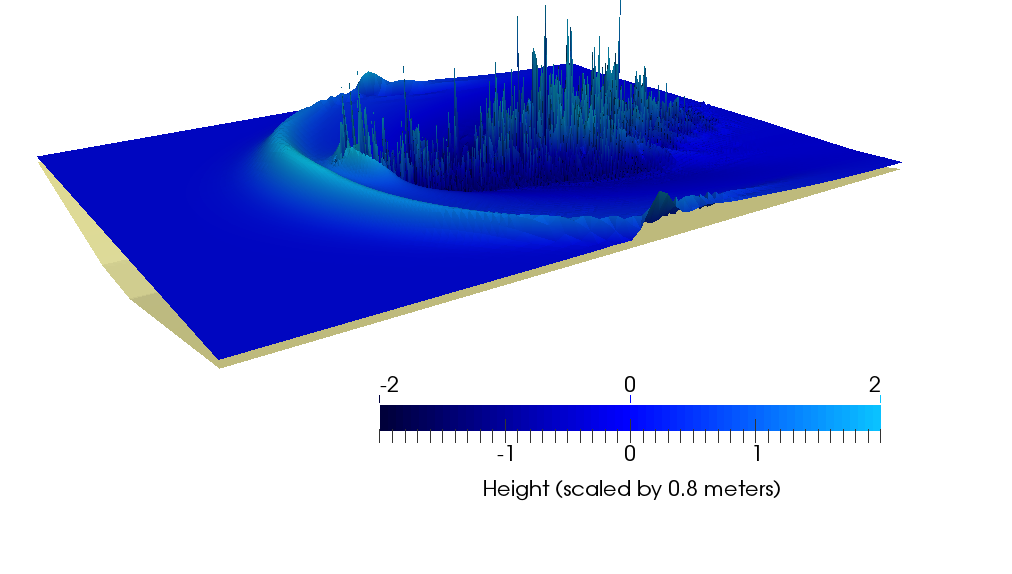
\includegraphics[height=4.8cm]{Instabilities.png}
			\caption{Instabilities with Crank-Nicholson time-stepping method}
		\end{minipage}
		\hspace{10pt}
		\begin{minipage}[t]{0.5\linewidth}
			\centering
			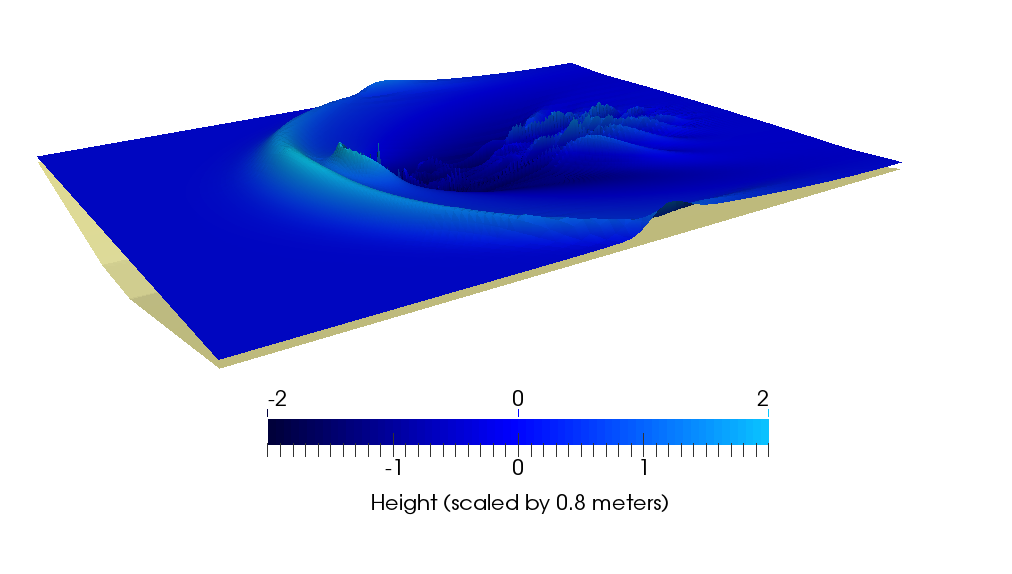
\includegraphics[height=4.8cm]{InstabilitiesCorrection.png}
			\caption{Result with Crank-Nicholson and stabilization with $c_f = 0.1$}
		\end{minipage}
	\end{figure}
		
\subsection{Assessment of the code: the solitary wave test}	
	One of the characteristic of the Peregrine system is that it admits a stationary solution that can be computed numerically. An interesting way to assess the code is therefore to compare that soliton with the solution of our code with this stationary solution as initial condition. We used D. DUTYKH's Matlab code to compute the following stationary solution: 
	\begin{figure}[!h]
		\centering
		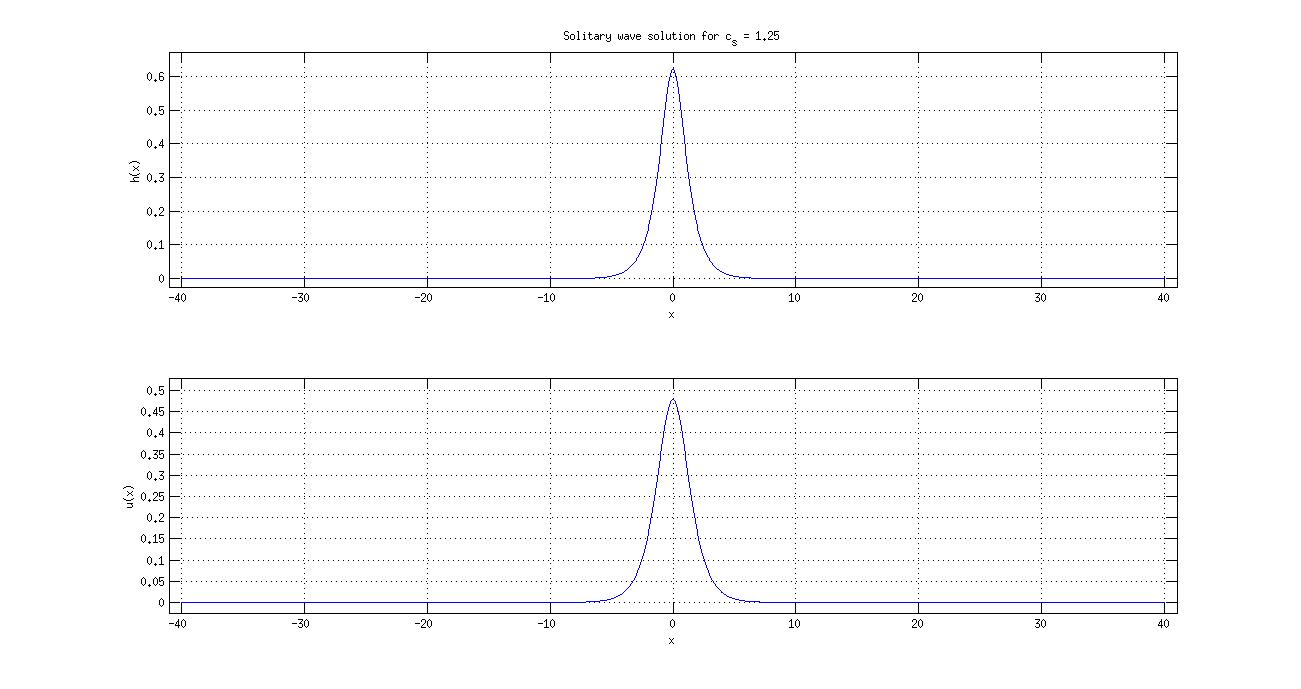
\includegraphics[height=6.5cm]{PeregrineSolitonSolution.jpg}
		\caption{Solitary solution (velocity $\mathbf{u}$ and free surface $\eta$)}
	\end{figure}		
			
	For different time stepping methods and using or no stabilization with different coefficients $c_f$, we compute the solution for different time step values $dt$ and compare it to the initial condition after a fixed final time step, during which the soliton moved of about 25 meters. 
	\begin{figure}[!h]
		\centering
		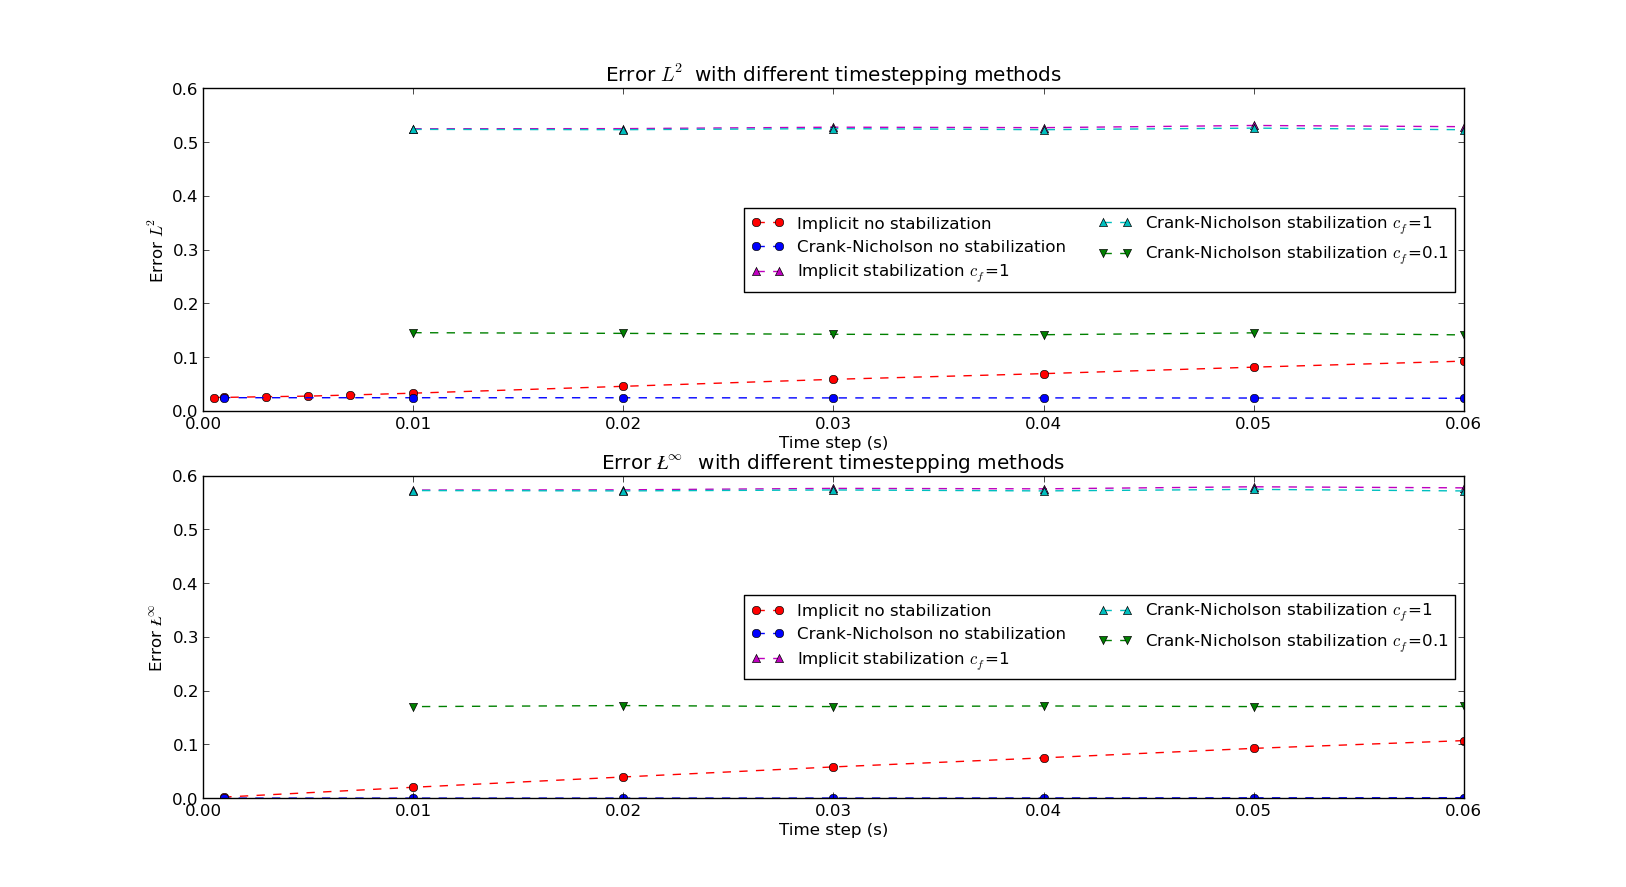
\includegraphics[height=8cm]{ErrorL2L801.png}
		\caption{Computation of the error $\mathbb{L}^2$ and $\mathbb{L}^{\infty}$}
	\end{figure}
	
	\begin{figure}[!h]
		\centering
		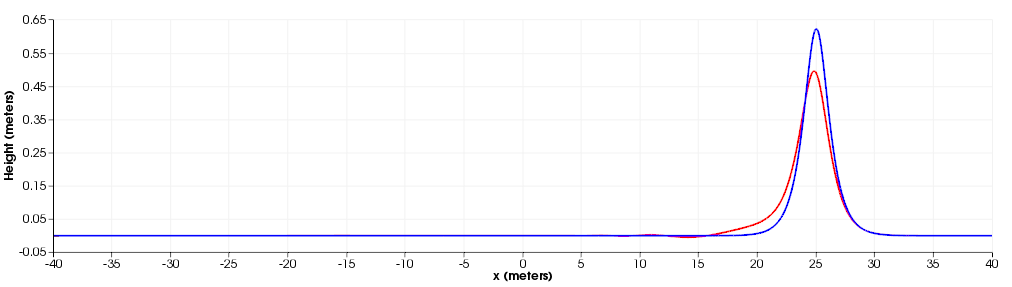
\includegraphics[height=4cm]{SolitonSolution.png}
		\caption{Computed soliton solution at final time for implicit and Crank-Nicholson time stepping methods}
	\end{figure}
	
	The Crank-Nicholson time stepping method gives good results, with an $\mathbb{L}^2$-error and an $\mathbb{L}^{\infty}$-error inferior as $3\%$, whereas the implicit time stepping method generates dissipation with an error $\mathbb{L}^2$ which increases with the time step. The stabilization induces more important errors for the mesh used here is not very refined. The size of the cells is here fixed for a computational reason (the Matlab results need to be read by FEniCS through a Python code). However in the real simulations, we use a more refined mesh which reduces the impact of stabilization as we can see in the following part. 
				
\subsection{Simulations and results}\label{Results}
	The following simulations were run using the following physical parameters (scaled for the simulation). For computational time issues, the mesh is on refined along the object trajectory and on one half of the pool.\\
	\begin{minipage}[t]{0.5\linewidth}
		\vspace{0pt}
		\begin{tabular}{|l|r|}
			\hline
			Pool's dimensions & $64\times50$ m$^2$	\\
			\hline
			Pool's maximal depth & $2$ m \\
			\hline
			Object's horizontal dimensions & $4\times6$ m$^2$\\
			\hline
			Object's maximal height & 0.8 m\\
			\hline
			Object's maximal velocity & 5.2 ms$^{-1}$\\
			\hline
			time step $dt$ & 0.03 s \\
			\hline		
			Final time T & 12.5 s\\
			\hline
			$\lambda_0$ & 20 m \\
			\hline
			$h_0$ & 2 m\\
			\hline
			$a_0$ & 0.8 m\\
			\hline
		\end{tabular}
		\captionof{table}{Values of parameters used in the numerical simulations}
	\end{minipage}
	\hfill
	\begin{minipage}[t]{0.5\linewidth}
		\vspace{0pt}
		\centering
		\includegraphics[height=5cm]{MeshandPool.png}
		\captionof{figure}{Mesh and dimensions of the pool}
	\end{minipage}
	\linebreak
	\begin{figure}[!h]
		\begin{minipage}[t]{0.5\linewidth}
			\centering
			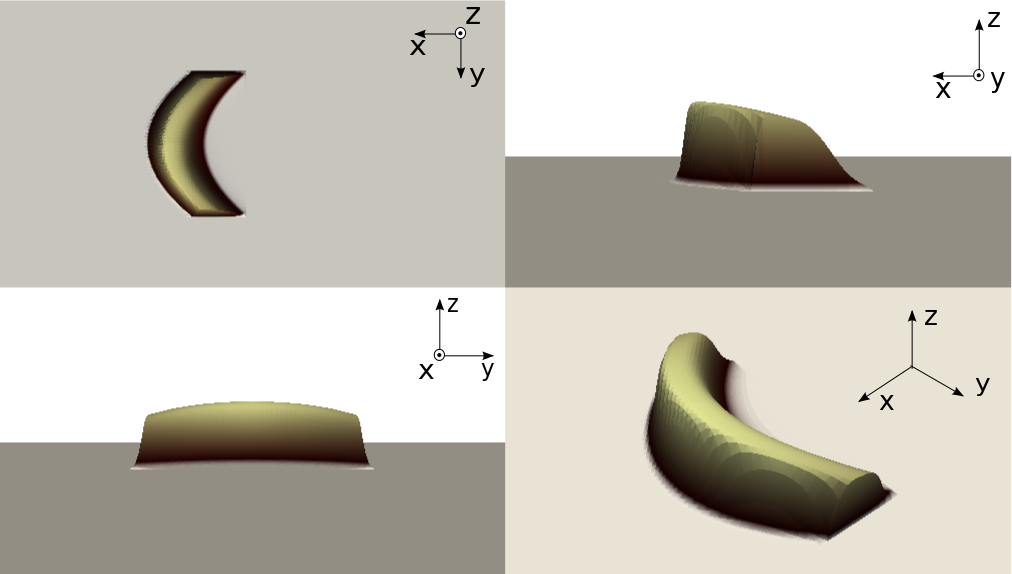
\includegraphics[height=4.5cm]{ObjectUsedModified.png}
			\caption{Object from different angles}
		\end{minipage}
		\hspace{10pt}
		\begin{minipage}[t]{0.5\linewidth}
			\centering
			\includegraphics[height=4.5cm]{ObjectTraj.png}
			\caption{Trajectory of the object (with real dimensions)}
		\end{minipage}
	\end{figure}

Thereafter are the results with different time stepping methods and using or not stabilization. The three pictures per simulation correspond to the times 4.5 s, 9 s and 12 s.
\begin{itemize}
	\item Crank-Nicholson time stepping method without stabilization
	\begin{figure}[!h]
		\begin{minipage}[t]{0.3\linewidth}
			\centering
			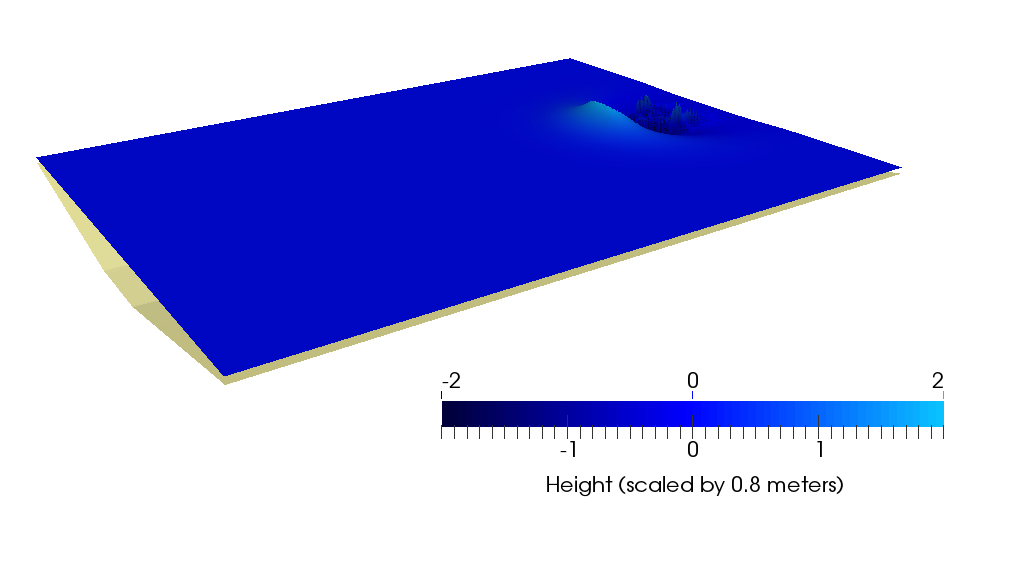
\includegraphics[width=5.5cm]{CNNoStabilized150.png}
		\end{minipage}
		\begin{minipage}[t]{0.3\linewidth}
			\centering
			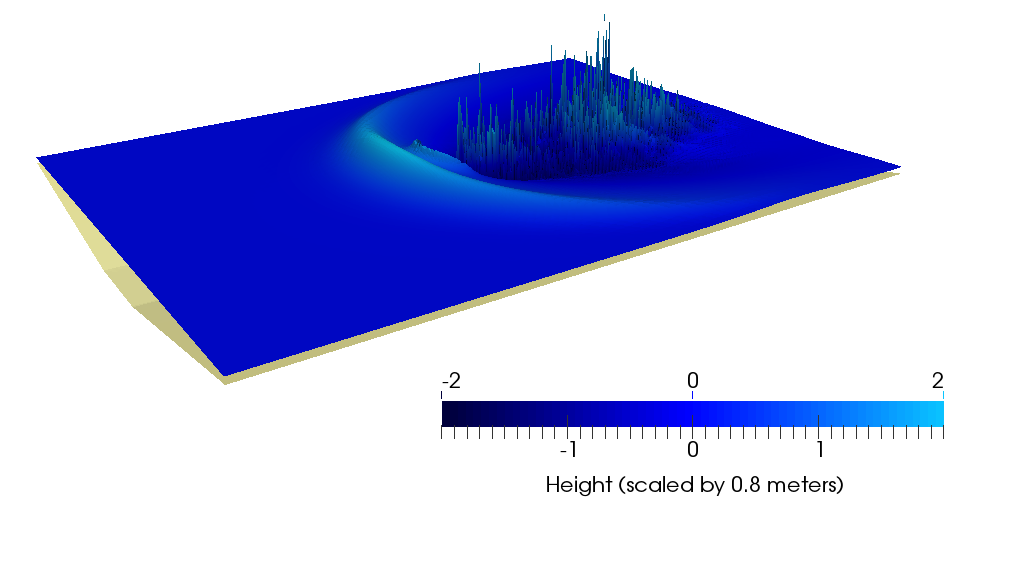
\includegraphics[width=5.5cm]{CNNoStabilized300.png}
		\end{minipage}
		\begin{minipage}[t]{0.3\linewidth}
			\centering
			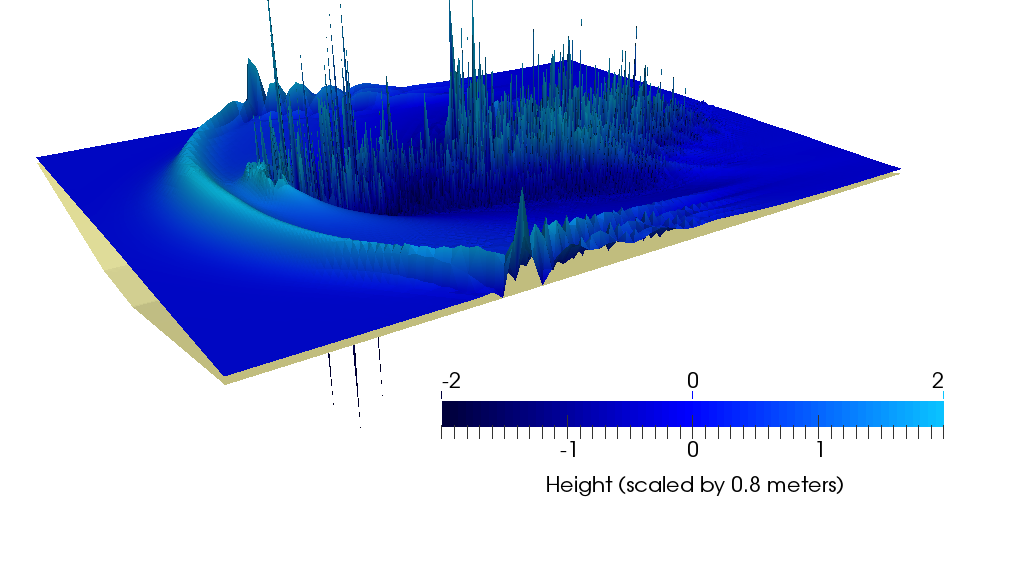
\includegraphics[width=5.5cm]{CNNoStabilized400.png}
		\end{minipage}
	\end{figure}
	\item Implicit time stepping method without stabilization
	\begin{figure}[!h]
		\begin{minipage}[t]{0.3\linewidth}
			\centering
			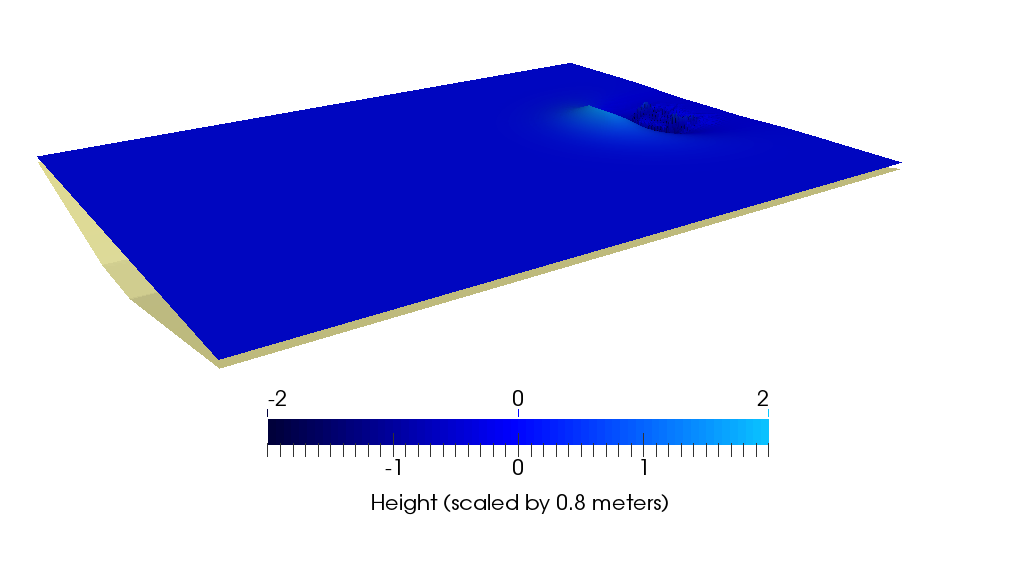
\includegraphics[width=5.5cm]{ImplicitNoStabilized150.png}
		\end{minipage}
		\begin{minipage}[t]{0.3\linewidth}
			\centering
			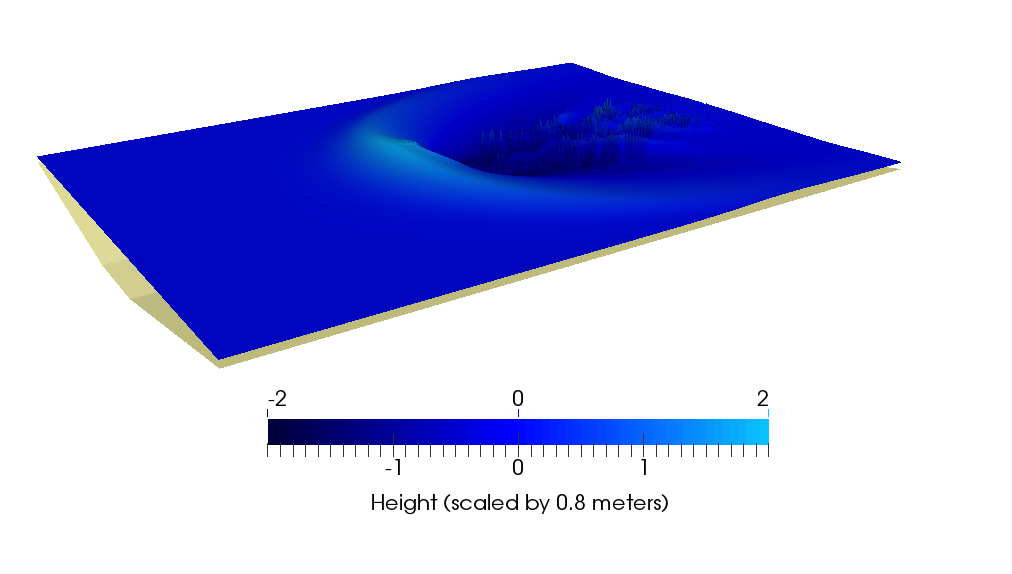
\includegraphics[width=5.5cm]{ImplicitNoStabilized300.png}
		\end{minipage}
		\begin{minipage}[t]{0.3\linewidth}
			\centering
			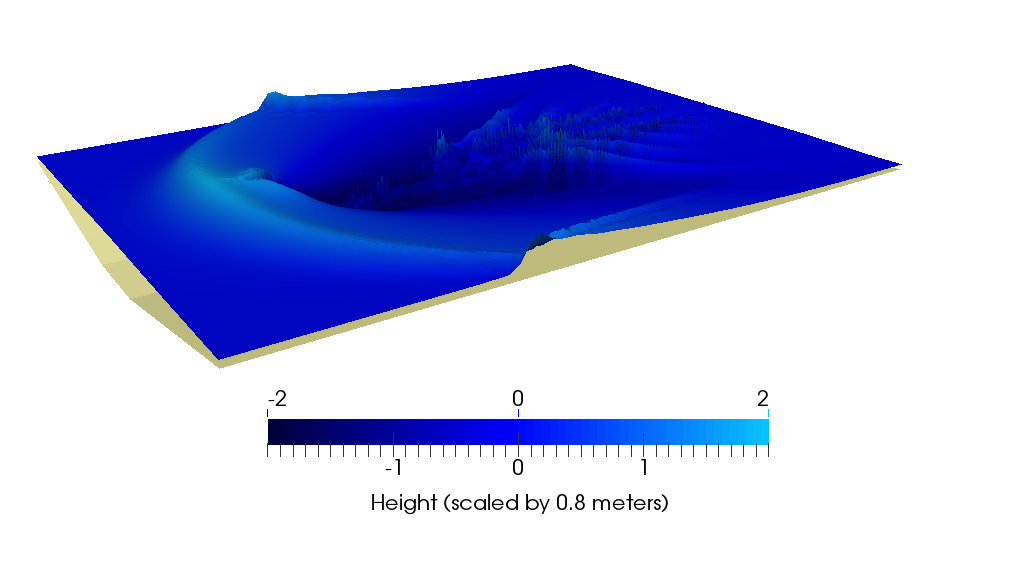
\includegraphics[width=5.5cm]{ImplicitNoStabilized400.png}
		\end{minipage}
	\end{figure}
	\item Crank-Nicholson time stepping method with stabilization ($c_f=0.1$)
	\begin{figure}[!h]
		\begin{minipage}[t]{0.3\linewidth}
			\centering
			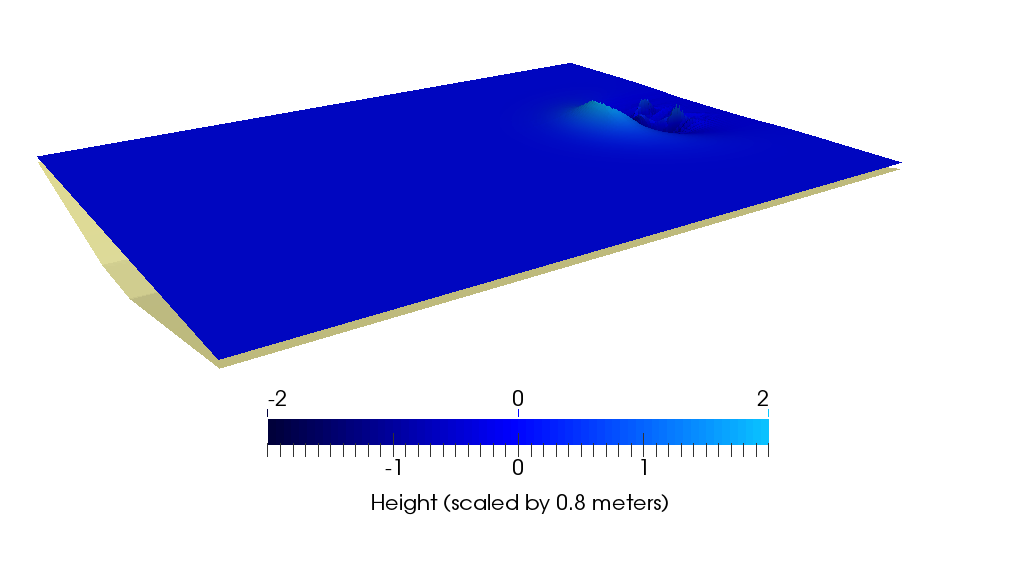
\includegraphics[width=5.5cm]{CNStabilized150.png}
		\end{minipage}
		\begin{minipage}[t]{0.3\linewidth}
			\centering
			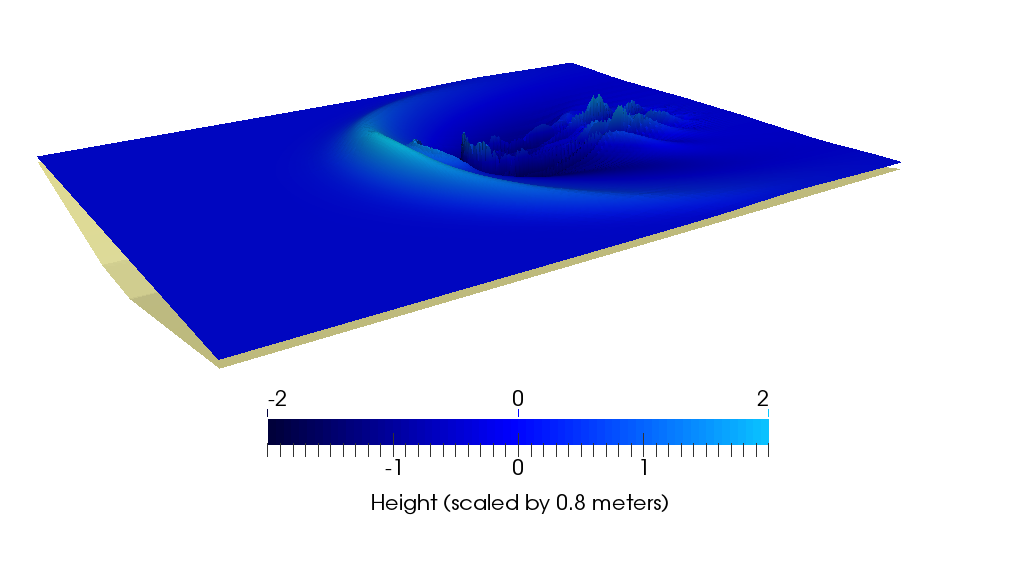
\includegraphics[width=5.5cm]{CNStabilized300.png}
		\end{minipage}
		\begin{minipage}[t]{0.3\linewidth}
			\centering
			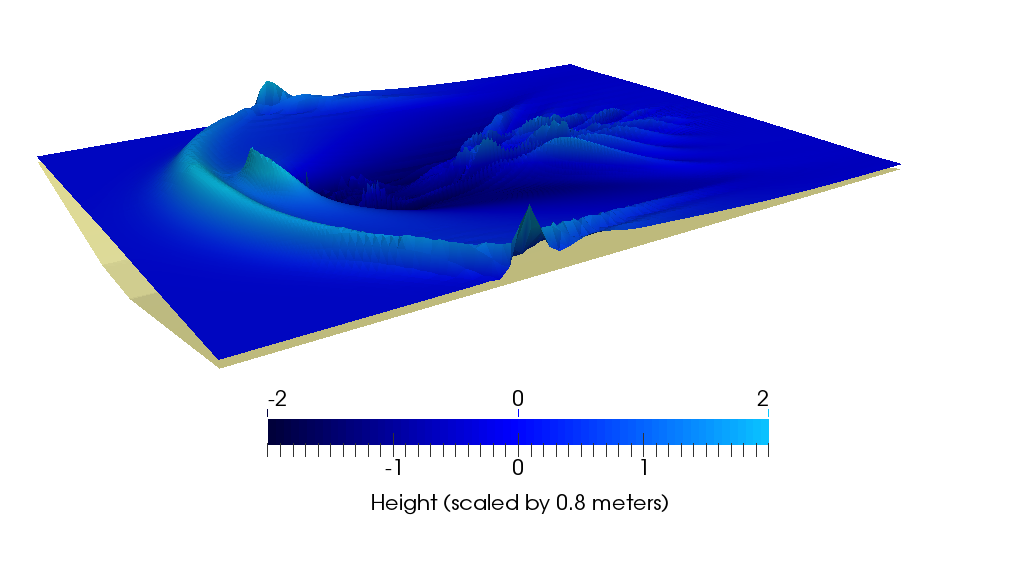
\includegraphics[width=5.5cm]{CNStabilized400.png}
		\end{minipage}
	\end{figure}
	\item Crank-Nicholson time stepping method with stabilization ($c_f=1$)
	\begin{figure}[!h]
		\begin{minipage}[t]{0.3\linewidth}
			\centering
			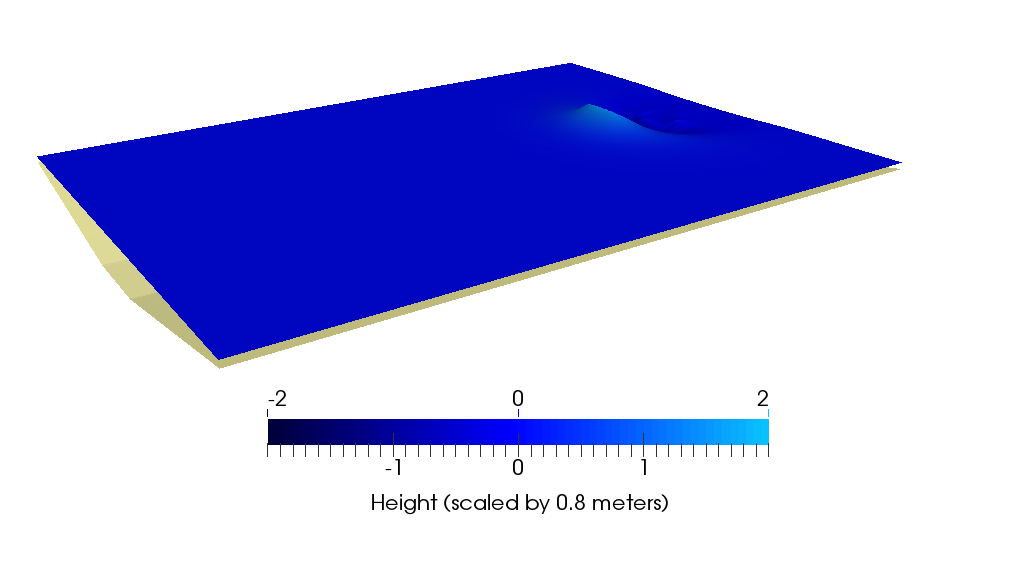
\includegraphics[width=5.5cm]{CNStabilized1_150.png}
		\end{minipage}
		\begin{minipage}[t]{0.3\linewidth}
			\centering
			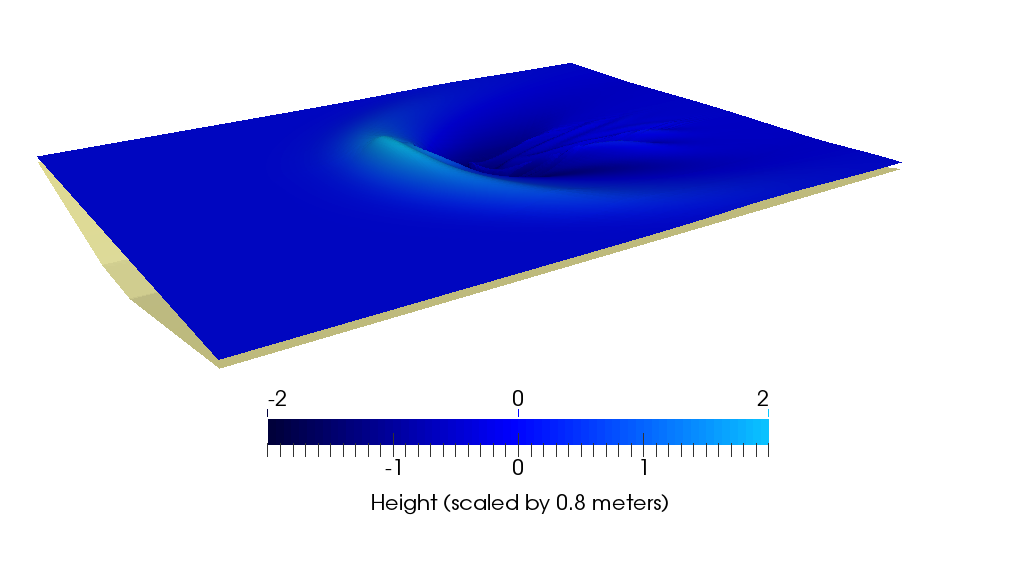
\includegraphics[width=5.5cm]{CNStabilized1_300.png}
		\end{minipage}
		\begin{minipage}[t]{0.3\linewidth}
			\centering
			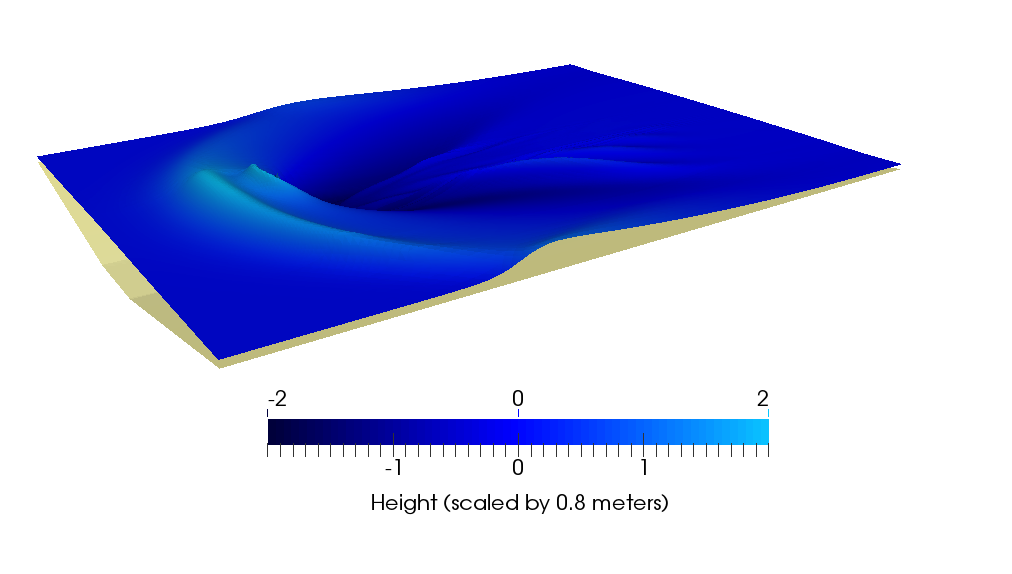
\includegraphics[width=5.5cm]{CNStabilized1_400.png}
		\end{minipage}
	\end{figure}
\end{itemize}

The stabilized simulation show less instabilities in the wake of the object, but if the stabilization coefficient $c_f$ is too big, the impact on the wave is important (last simulation). However, with $c_f=0.1$, we see that we can avoid the instabilities without dissipating the created wave. As seen in the solitary wave simulation, the implicit time stepping method induces also an important dissipation.

\pagebreak
	
\section{Optimization}
	In this part we will focus on the optimization of the moving object so as to minimize a given functional characterizing the quality of the final water wave.
	\begin{equation}
		\inf_{\zeta_0 \in U_{ad}}\left\{J(\zeta_0)\ = \int_0^T {\int_{\Omega}{\! j(\eta(t), \mathbf{u}(t), \zeta_0) \: \mathrm{dx}} \: \mathrm{dt}} \right\}
	\end{equation}
	The set $U_{ad}$ of the admissible shapes includes only objects located at the central lane of the pool and with a determined maximal width and height. Therefore, $U_{ad} = \{\zeta_0 \in \mathbb{H}^1(\Omega), \zeta_{min} \leq \zeta_0 \leq \zeta_{max}   \}$.
	\begin{figure}[!h]
		\centering
		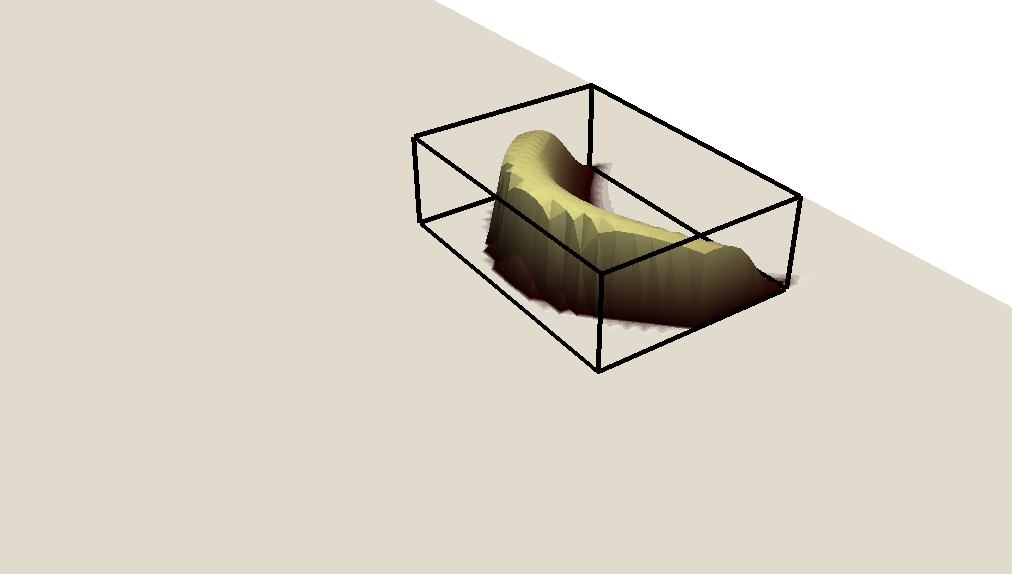
\includegraphics[height=5cm]{ObjectBoundaries.png}
		\caption{Set of admissible shapes}
	\end{figure}

\subsection{Coupling with the transport equation}
	In the Peregrine system, our optimization parameter $\zeta_0$ appears as a time-dependent forcing function $\zeta(\mathbf{x}, t)$.
	\begin{center}
		$\left\lbrace
			\begin{array}{rll}
				\displaystyle \mathbf{u}_t + \nabla \eta + \epsilon (\mathbf{u} \cdot \nabla)\mathbf{u} - \sigma^2\frac{D + \epsilon \zeta}{2}\nabla (\nabla \cdot ((D + \epsilon \zeta) \mathbf{u}_t)) & + \sigma^2 \dfrac{(D + \epsilon \zeta)^2}{6}\nabla (\nabla \cdot \mathbf{u}_t)  &  \\
				& \qquad \qquad -  \sigma^2\dfrac{D + \epsilon \zeta}{2}\nabla \zeta_{tt}  & =  0 \\
				& \displaystyle \eta_t+\zeta_t + \nabla \cdot [(D + \epsilon \zeta+\epsilon\eta)\mathbf{u}] & =  0
			\end{array}
		\right.$
	\end{center}
	However we know explicitly the dependency in time of $\zeta$, as it is the transported initial object $\zeta(\mathbf{x},t) =  \zeta_0(\mathbf{x} - \epsilon \int_0^t{\! \mathbf{U}(s) \: \mathrm{ds}})$ where $\mathbf{U}(t)$ is the dimensionless velocity of the object, that we consider fixed. A first approach to overcome this difficulty will be to couple the Peregrine system with the transport equation verified by the object, so as to make explicitly appear the initial shape $\zeta_0$ as the control of our system.
	
\subsubsection{Complete system}
	The coupling between the Peregrine system and the transport equation leads us to the following system:
	\begin{align}
		\mathbf{u}_t + \nabla \eta + \epsilon (\mathbf{u} \cdot \nabla)\mathbf{u} - \sigma^2\frac{h}{2}\nabla (\nabla \cdot (h \mathbf{u}_t)) + \sigma^2 \frac{h^2}{6}\nabla (\nabla \cdot \mathbf{u}_t) - \sigma^2\frac{h}{2}\nabla \zeta_{tt}  &= 0\\
		\eta_t+\zeta_t + \nabla \cdot [(h+\epsilon\eta)\mathbf{u}] &= 0 \\
		\zeta_t + \epsilon \mathbf{U} \cdot \nabla \zeta &= 0\\
		\zeta(x,y,t=0) &= \zeta_0(x,y)
	\end{align}
	As the transport equation does not depend on the Peregrine system, we can solve each system separately step by step. The main advantage of this method is that it will allows us to use directly the optimization framework proposed by the library \textit{Dolfin-Adjoint} as long as we use \textit{FEniCS} and \textit{Dolfin}  to solve the transport equation. Indeed, \textit{Dolfin-Adjoint} makes it very easy to do optimization with respect to an initial condition parameter or a time-independent parameter. However, it implies that we have to solve the transport equation using finite elements, which raises the problem of the instability of hyperbolic equations with finite element method. To be able to optimize correctly the shape of the object, we need however to transport this shape along the object trajectory with a good accuracy. A simple implicit scheme as:
	\begin{equation}\label{TransportSimple}
	\left\lbrace
	\begin{split}
		&\int_{\Omega}{\! \tau \frac{\zeta^{n+1} - \zeta^n}{\Delta t}}  -   \epsilon \int_{\Omega}{\! \nabla \tau \cdot  \mathbf{U}^{n+1}  \zeta^{n+1}}\\
		&\zeta = 0 \quad \mathrm{on} \quad \partial \Omega
		\end{split}
		\right.
	\end{equation} 
	is not enough and the following part will therefore present a Taylor-Galerkin method used to solve this equation with a better accuracy. The lector is invited to see \cite{Transport} for more details on that topic. 
				
\subsubsection{Stabilization of the transport equation using Taylor-Galerkin method}
	We detail here the method used to establish the second-order Taylor-Galerkin scheme. Let $\Delta t$ be a small time-step and $\theta \in [0,1]$ the time-stepping method used, we have:	
	\begin{align}
		\displaystyle \frac{\zeta^{n+1} - \zeta^n}{\Delta t} = \left(\frac{\partial \zeta}{\partial t} \right)^n + \frac{\Delta t}{2} \left(\frac{\partial^2 \zeta}{\partial t^2} \right)^{n+\theta} + O(\Delta t^2)
	\end{align}
	using the transport equation
	\begin{equation}
		\displaystyle \frac{\partial \zeta}{\partial t} = - \epsilon \mathbf{U} \cdot \nabla \zeta, \qquad \displaystyle \frac{\partial^2 \zeta}{\partial t^2} = - \epsilon \frac{\partial \mathbf{U}}{\partial t} \cdot \nabla \zeta - \epsilon \mathbf{U} \cdot \nabla \frac{\partial \zeta}{\partial t}
	\end{equation}
	we get:
	\begin{align}
		\displaystyle \frac{\zeta^{n+1} - \zeta^n}{\Delta t} =- \epsilon \mathbf{U}^n \cdot \nabla \zeta^n - \frac{\epsilon \Delta t}{2} \left(\frac{\partial \mathbf{U}}{\partial t} \cdot \nabla \zeta^{n+\theta} - \epsilon \mathbf{U}^{n+\theta} \cdot \nabla (\mathbf{U}^{n+\theta} \cdot \nabla \zeta^{n+\theta})\right) + O(\Delta t^2)
	\end{align}
	which lead us to the following weak formulation: $\forall \tau \in \mathbb{H}^1_0(\Omega)$,
	\begin{align}
		\displaystyle \int_{\Omega}{\! \tau \frac{\zeta^{n+1} - \zeta^n}{\Delta t}}  -   \epsilon \int_{\Omega}{\! \nabla \tau \cdot  \mathbf{U}^n  \zeta^n} - \frac{\epsilon \Delta t}{2} \int_{\Omega}{\! \nabla \tau \cdot \frac{\partial \mathbf{U}}{\partial t} \zeta^{n+\theta}}
		 +  \frac{\epsilon^2 \Delta t}{2} \int_{\Omega}{\! (\nabla \tau \cdot \mathbf{U})(\nabla \zeta^{n+\theta} \cdot \mathbf{U}^{n+\theta})} = 0
	\end{align}
	Will the same method, a Taylor series expanded to the order 3 would give us the following:  $\forall \tau \in \mathbb{H}^1_0(\Omega)$,
	\begin{align*}
		& \displaystyle \int_{\Omega}{\! \tau \frac{\zeta^{n+1} - \zeta^n}{\Delta t}}  -   \epsilon \int_{\Omega}{\! \nabla \tau \cdot  \mathbf{U}^n  \zeta^n} + \frac{\Delta t}{2}\left( - \epsilon \int_{\Omega}{\! \nabla \tau \cdot \frac{\partial \mathbf{U}}{\partial t} \zeta^{n+\theta}}
		 +  \epsilon^2 \int_{\Omega}{\! (\nabla \tau \cdot \mathbf{U})(\nabla \zeta^{n+\theta} \cdot \mathbf{U}^{n+\theta})}\right) \\
		 & -\frac{\Delta t^2}{6}\left(\epsilon \int_{\Omega}{\! \nabla \tau \cdot \frac{\partial^2 \mathbf{U}}{\partial t^2} \zeta^{n+\theta}} -2\epsilon^2 \int_{\Omega}{\! (\nabla \tau \cdot \frac{\partial \mathbf{U}}{\partial t})(\nabla \zeta^{n+\theta} \cdot \mathbf{U}^{n+\theta})} -\epsilon^2 \int_{\Omega}{\! (\nabla \zeta^{n+\theta} \cdot \frac{\partial \mathbf{U}}{\partial t})(\nabla \tau \cdot \mathbf{U}^{n+\theta})}\right) \\
		 & -\frac{\Delta t}{6} \epsilon^2 \int_{\Omega}{\! (\nabla \tau \cdot \mathbf{U})(\nabla (\zeta^{n+1} -  \zeta^n) \cdot \mathbf{U}^{n+\theta})}  = 0
	\end{align*}	
	The results of those different methods used are shown in the Figure \ref{Transport}. All the simulations stop before the object reaches the right boundary and we use therefore homogeneous Dirichlet boundary conditions to solve the different weak formulations. We notice immediately the important dissipation in the implicit scheme \eqref{TransportSimple}, which justify the need of another weak formulation. The Taylor-Galerkin schemes have been computed with $\theta = 0.5$. The second order scheme shows the best accuracy among all the schemes tested. If this scheme keeps the height of the object none of the following schemes seems to be able to keep the steepness of the leading edge.
	\begin{figure}
		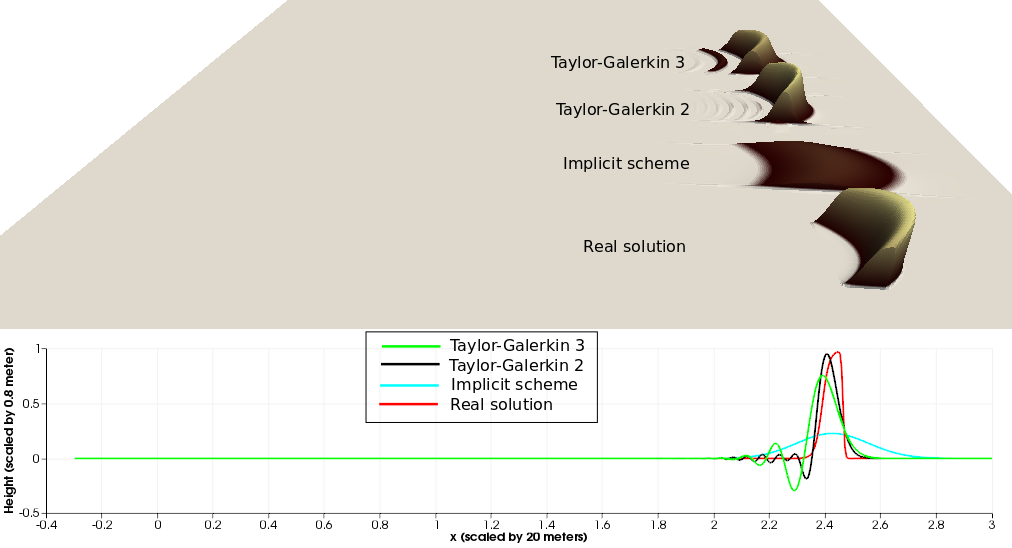
\includegraphics[height=8cm]{TransportComparison.png}
		\caption{Simulation of the transport equation with different numerical schemes in 2D and with a cross-section}
		\label{Transport}
	\end{figure}

\subsection{First optimization without energy consideration}
\subsubsection{Functional to minimize}
	To test the optimization process, the first functional which will be used to assess the wave is the $\mathbb{H}^1$ norm of the height of the free surface  $\eta$ at a final time $T$ over a specific domain $\omega$, on which the surfer is supposed to move on the wave. This functional allows to maximise both the height and the steepness of the generated wave at the final time step:
	\begin{minipage}[c]{0.5\linewidth}
		\vspace{0pt}
		\centering
		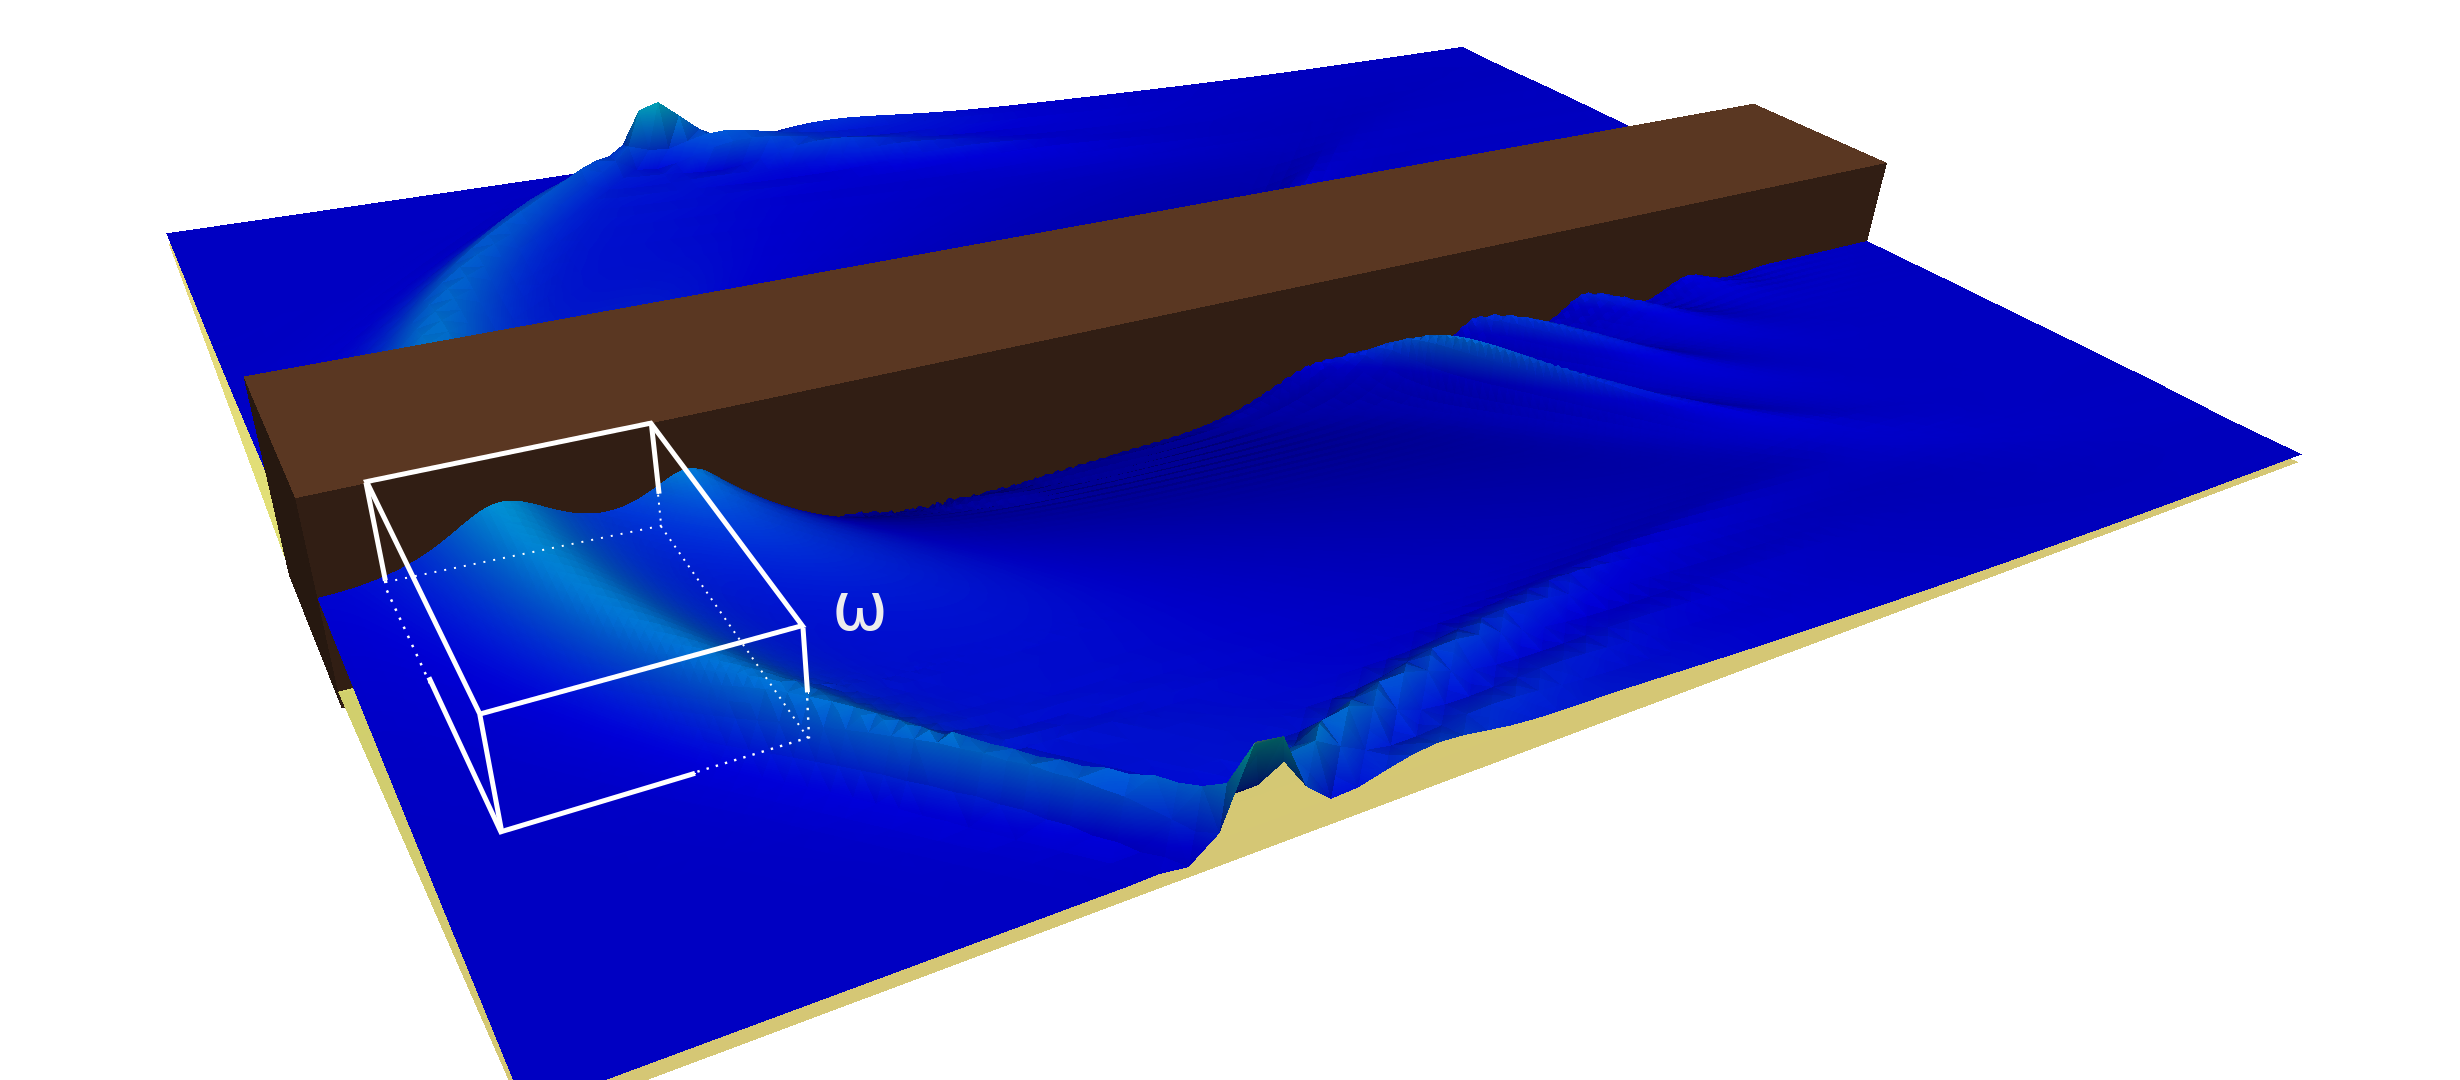
\includegraphics[height=3cm]{OptimizationDomain}
		\captionof{figure}{Domain $\omega$ on which the wave is assessed}
	\end{minipage}	
	\begin{minipage}[c]{0.5\linewidth}
		\vspace{0pt}
		\begin{equation}
			j(\eta(T),\zeta_0) = - \frac{1}{2T}(|\eta(T)|^2 + |\nabla \eta(T)|^2) \mathds{1}_{\omega}
		\end{equation}
	\end{minipage}


	
	

\subsubsection{Results and convergence}		
	To run this optimization without having to derive the adjoint system and to compute the gradient, we use the optimization framework of \textit{Dolfin-Adjoint}, coupled with \textit{Ipopt} through a Python code.	\textit{Ipopt} (short ``Interior Point OPTimizer") is a software package for large-scale non-linear optimization, using an interior point method (\cite{IPOPT}). 
	\begin{figure}[!h]
		\begin{minipage}[t]{0.5\linewidth}
			\centering
			\includegraphics[height=4.8cm]{OPT-Pyipopt.png}
			\caption{Convergence of the functional value}
		\end{minipage}
		\hspace{10pt}
		\begin{minipage}[t]{0.5\linewidth}
			\centering
			\includegraphics[height=4.8cm]{OptimalShapePyipopt.png}
			\caption{Object's shape at final iteration using Pyipopt}
			\label{OptimalShapePyipot}
		\end{minipage}
	\end{figure}
	
	The result found by \textit{Ipopt} is a single bloc of maximal height and width allowed in the set of admissible shape. The optimization of the shape tends to same result using directly \textit{Dolfin-Adjoint} and a truncated Newton algorithm, but with a slower convergence. If this shape seems minimalist at first sight and not the one desired, the comparison of the wave created by this object and the one used in the previous simulations (section \ref{Results})clarify the situation (Figure \ref{WaveBloc}): if the generated wave is bigger and steeper, we can see a lot of perturbations in the wake of the bloc object: moving a bloc under the water uses a lot of energy, lost in the perturbations in the wake. The criteria used (height and steepness of the wave) are therefore unsatisfactory and an energy criterion must be consider to find an acceptable solution to this problem.	
	\begin{figure}[!h]
		\begin{minipage}[t]{0.5\linewidth}
			\centering
			\includegraphics[height=4.8cm]{WaveSmooth.png}
			\caption{Wave generated by the initial object}
		\end{minipage}
		\hspace{10pt}
		\begin{minipage}[t]{0.5\linewidth}
			\centering
			\includegraphics[height=4.8cm]{WaveBloc.png}
			\caption{Wave generated by the bloc object}
			\label{WaveBloc}
		\end{minipage}
	\end{figure}

\subsection{Energetic consideration}

	To find a good compromise between the size of the created wave and the energy required to pull the object, we need to take an other factor in account: the resistance of the object while it is moving under the water. An optimal shape will allow the object to create a big wave, but with a weak resistance whilst it is moving.
	
\subsubsection{Recovering the pressure in the Peregrine system}		
	As we are using a two dimensional model, one way to evaluate the forces on the object is to recover the pressure from Euler equations, used to derived the Peregrine system in the section \ref{Part1}.
				
	Using the equation \eqref{Pressure} for $ z = -h$, and the equation \eqref{AverageVelocity2}, we get:
	\begin{equation}
		P(z=-h) = \epsilon \sigma^2(-h\nabla \cdot (h \mathbf{u}_t) + \frac{h^2}{2} \nabla \cdot \mathbf{u}_t) - \epsilon \sigma^2 h \zeta_{tt} + \epsilon \eta + h + O(\epsilon\sigma^4, \epsilon^2 \sigma^2)
	\end{equation}	
	Knowing the pressure on the seabed, we now want to find the total force applied on the object.	Let $t$ be a fixed time and $\mathbf{n}$ be the unit vector normal to surface $\Sigma(t)_{object} = \{(x,y,z), z = - h(x,y,t), \zeta(x,y,t)\neq 0 \} $ and $\Omega(t)_{object} = \{(x,y), \zeta(x,y,t)\neq 0 \} $ . The projection of that vector on the horizontal plan is the vector $\hat{\mathbf{n}} = - \dfrac{\nabla h(x,y,t)}{|\nabla h(x,y,t)|}$. The total horizontal force applied on the object at time $t$ is therefore the following: 
	\begin{align*}
		\mathbf{F}(t) &= \int_{\Sigma(t)_{object}}{\! P(\hat{x}, \hat{y}) (-\hat{\mathbf{n}})(\hat{x},\hat{y}) \: \mathrm{d\hat{x}}\:\mathrm{d\hat{y}}}\\
		 & = - \int_{\Omega(t)_{object}}{\! P(-h(x,y,t)) \hat{\mathbf{n}}(h(x,y,t)) |-\nabla h(x,y,t)| \: \mathrm{dx}\:\mathrm{dy}}\\
		 & = \int_{\Omega(t)_{object}}{\! P(-h(x,y,t)) \nabla h(x,y,t) \: \mathrm{dx}\:\mathrm{dy}}\\
		 & = \epsilon \int_{\Omega}{\! P(-h(x,y,t)) \nabla \zeta(x,y,t) \: \mathrm{dx}\:\mathrm{dy}}
	\end{align*}	
	With this formula, we are now able to evaluate the constraints on the moving object over time and therefore to minimize them.
	
\textbf{	\textcolor{red}{ADD GRAPHICS AND PICTURES OF THE PRESSURE AND THE FORCE - COMMENT INSTABILITIES OBSERVED FOR THE BLOCK OBJECT}	}

\subsection{Derivation of the adjoint system}
	To avoid the lost of information caused by the inaccuracy of the numerical resolution of the transport equation, the alternative is to derive and code ourself a gradient method using the explicit expression of $\zeta(\mathbf{x},t)$ so as to get rid of \textit{Dolfin-Adjoint} constraints. The following calculations explain a method to compute the adjoint and the gradient of a functional depending only of the final free surface, for an implicit time stepping method and without added stabilization, using Lagrange multipliers. It can easily be extended to other functionals, time stepping methods and cases with stabilization.
	
	Calling $(\mathbf{v}^N, \xi^N), ... (\mathbf{v}^0, \xi^0)$ the Lagrange multipliers associated with $(\mathbf{u}^N, \eta^N), ... (\mathbf{u}^0, \eta^0)$, we can now define the Lagrangian $\mathcal{L} $ of our problem: 
		
		\begin{equation}
			\begin{split}
				&\mathcal{L}(\zeta_0, (\mathbf{u}^N, \eta^N), ... (\mathbf{u}^0, \eta^0), 	(\mathbf{v}^N, \xi^N), ... (\mathbf{v}^0, \xi^0))	= J(\zeta_0) + \sum_{k=0}^{k=N-1} \left[ \int_{\Omega} \! \frac{\mathbf{u}^{k+1} - \mathbf{u}^k}{\Delta t} \cdot	\mathbf{v}^{k+1} \: \mathrm{dx} \right. \\
				 &\quad - \int_{\Omega} \! \eta^{k+1} \; (\nabla \cdot \mathbf{v}^{k+1}) \: \mathrm{dx} + \epsilon \! \int_{\Omega} \! (\mathbf{u}^{k+1} \cdot \nabla ) \mathbf{u}^{k+1} \cdot	\mathbf{v}^{k+1} \: \mathrm{dx} + \displaystyle\int_{\Omega}\! \frac{\eta^{k+1} - \eta^{k}}{\Delta t} \; \xi^{k+1} \: \mathrm{dx} + \int_{\Omega}\! \zeta^{k+1}_t \; \xi^{k+1} \: \mathrm{dx} \\
				 &\quad-\int_{\Omega}\! \nabla \xi^{k+1} \; \cdot [(D + \epsilon \zeta^{k+1} + \epsilon \eta^{k+1}) \mathbf{u}^{k+1}] \:	\mathrm{dx} + \frac{\sigma^2}{2} \! \int_{\Omega} \! \zeta^{k+1}_{tt}  \; (\nabla \cdot( (D+\epsilon \zeta^{k+1}) \mathbf{v}^{k+1})) \: \mathrm{dx} \\ 
					&\quad+ \frac{\sigma^2}{2} \! \int_{\Omega} \!  (\nabla \cdot ((D + \epsilon \zeta^{k+1})	\frac{\mathbf{u}^{k+1} - \mathbf{u}^{k}}{\Delta t})) \; (\nabla \cdot ((D + \epsilon \zeta^{k+1}) \mathbf{v}^{k+1})) \: \mathrm{dx} \\
					&\quad\left. - \frac{\sigma^2}{6} \! \int_{\Omega} \! (\nabla 
					\cdot \frac{\mathbf{u}^{k+1} - \mathbf{u}^{k}}{\Delta t}) \; (\nabla  \cdot	((D + \epsilon \zeta^{k+1})^2  \mathbf{v}^{k+1})) \: \mathrm{dx} \right]	
			\end{split}
		\end{equation}
		where we denoted $\zeta^k(\mathbf{x}, t) = \zeta_0(\mathbf{x}-\mathbf{f}(t^k),y)$ with $\mathbf{f}(t) = \int_0^t{\! \mathbf{U}(s) \: \mathrm{ds}}$ the trajectory of the object.
		
		Differentiating the Lagrangian with respect to the velocity and the height at each time step gives us the adjoint system: $\forall (\mathbf{u},\eta) \in \mathbb{V} \times \mathbb{H}^1(\Omega)$		
		\begin{equation}
			\begin{split}
				0 & = \int_{\Omega} \! \frac{\mathbf{v}^{N}}{\Delta t} \cdot	\mathbf{u} \: \mathrm{dx} + \epsilon \int_{\Omega} \! ((\mathbf{u} \cdot \nabla )\mathbf{u}^N + (\mathbf{u}^N \cdot \nabla )\mathbf{u}) \cdot 	\mathbf{v}^{N} \: \mathrm{dx} 	- \int_{\Omega} \! (\epsilon \eta^N + D + \epsilon \zeta^N) \mathbf{u} \cdot \nabla \xi^N \: \mathrm{dx} \\
				&\quad + \frac{\sigma^2}{2} \int_{\Omega} \! \nabla \cdot ((D + \epsilon \zeta^N) \mathbf{u})  \nabla \cdot \left(\frac{(D+ \epsilon \zeta^N)\mathbf{v}^N}{\Delta t}\right) \: \mathrm{dx} - \frac{\sigma^2}{6} \int_{\Omega} \! (\nabla \cdot \mathbf{u})  \nabla \cdot \left(\frac{(D+ \epsilon \zeta^N)^2 \mathbf{v}^N}{\Delta t}\right) \: \mathrm{dx} \\
				& + stabilization \\
				0 & = \int_{\Omega} \! \frac{\xi^{N}}{\Delta t} \eta \: \mathrm{dx} - \int_{\Omega} \! \eta (\nabla \cdot \mathbf{v}^N) \: \mathrm{dx} - \int_{\Omega} \! \epsilon \eta \mathbf{u}^N \cdot \nabla \xi^N \: \mathrm{dx} + \int_{\Omega} \! \frac{\partial j}{\partial \eta^N}(\eta^N) \eta + stabilization
			\end{split}			
		\end{equation}
		which gives us $(\mathbf{v}^N, \xi^N)$, and then for all $k<N$, we solve the following system backward in time: $\forall (\mathbf{u},\eta) \in \mathbb{V} \times \mathbb{H}^1(\Omega)$ 
		\begin{equation}
			\begin{split}
				0 & = \int_{\Omega} \! \frac{\mathbf{v}^{k} - \mathbf{v}^{k+1}}{\Delta t} \cdot	\mathbf{u} \: \mathrm{dx} + \epsilon \int_{\Omega} \! ((\mathbf{u} \cdot \nabla )\mathbf{u}^k + (\mathbf{u}^k \cdot \nabla )\mathbf{u}) \cdot 	\mathbf{v}^{k} \: \mathrm{dx} 	- \int_{\Omega} \! (\epsilon \eta^k + D + \epsilon \zeta^k) \mathbf{u} \cdot \nabla \xi^k \: \mathrm{dx} \\
				&\quad + \frac{\sigma^2}{2} \int_{\Omega} \! \nabla \cdot ((D + \epsilon \zeta^k) \mathbf{u})  \nabla \cdot \left(\frac{(D+ \epsilon \zeta^k)\mathbf{v}^k - (D + \epsilon \zeta^{k+1})\mathbf{v}^{k+1})}{\Delta t}\right) \: \mathrm{dx} \\
				&\quad - \frac{\sigma^2}{6} \int_{\Omega} \! (\nabla \cdot \mathbf{u})  \nabla \cdot \left(\frac{(D+ \epsilon \zeta^k)^2 \mathbf{v}^k - (D + \epsilon \zeta^{k+1})^2 \mathbf{v}^{k+1})}{\Delta t}\right) \: \mathrm{dx} + stabilization \\
				0 & = \int_{\Omega} \! \frac{\xi^{k} - \xi^{k+1}}{\Delta t} \eta \: \mathrm{dx} - \int_{\Omega} \! \eta (\nabla \cdot \mathbf{v}^k) \: \mathrm{dx} - \int_{\Omega} \! \epsilon \eta \mathbf{u}^k \cdot \nabla \xi^k \: \mathrm{dx} + stabilization
			\end{split}			
		\end{equation}
		Knowing the solution of the forward problem and the adjoint at each time step, we are now looking for an explicit formulation for the gradient of our functional $J(\zeta_0)$: $\forall \chi \in U_{ad}$
		\begin{equation*}
			\begin{split}
				<\!J'(\zeta_0),\chi\!> &= <\! \frac{\partial \mathcal{L}}{\partial \zeta_0}(\zeta_0, (\mathbf{u}^N, \eta^N), ... (\mathbf{u}^0, \eta^0), 	(\mathbf{v}^N, \xi^N), ... (\mathbf{v}^0, \xi^0)), \chi\!> \\
				&= \sum^{N}_{k=1} \left[ \int_{\Omega} \! <\!\frac{\partial\zeta^k}{\partial \zeta_0}, \chi\!> \xi^k \: \mathrm{dx} - \int_{\Omega} \! \epsilon <\!\frac{\partial\zeta_t^k}{\partial \zeta_0}, \chi\!> \mathbf{u}^k \cdot \nabla \xi^k \: \mathrm{dx} \right.\\
				& \quad + \frac{\epsilon \sigma^2}{2} \int_{\Omega} \! \nabla \cdot \left( <\!\frac{\partial\zeta^k}{\partial \zeta_0}, \chi\!> \frac{\mathbf{u}^k - \mathbf{u}^{k-1}}{\Delta t} \right) \nabla \cdot \left( (D + \epsilon \zeta^k) \mathbf{v}^k \right) \: \mathrm{dx} \\
				& \quad + \frac{\epsilon \sigma^2}{2} \int_{\Omega} \! \nabla \cdot \left((D+\epsilon \zeta^k)\frac{\mathbf{u}^k - \mathbf{u}^{k-1}}{\Delta t}\right) \nabla \cdot \left(<\!\frac{\partial\zeta^k}{\partial \zeta_0}, \chi\!> \mathbf{v}^k \right) \: \mathrm{dx} \\
				&  \quad - \frac{\epsilon \sigma^2}{3} \int_{\Omega} \! \nabla \cdot \left( \frac{\mathbf{u}^k - \mathbf{u}^{k-1}}{\Delta t} \right) \nabla \cdot \left( <\!\frac{\partial\zeta^k}{\partial \zeta_0}, \chi\!> (D + \epsilon \zeta^k) \mathbf{v}^k \right) \: \mathrm{dx} \\
				& \left. \quad + \frac{\sigma^2}{2}\int_{\Omega} \! <\!\frac{\partial\zeta_{tt}^k}{\partial \zeta_0}, \chi\!> \nabla \cdot \left( (D + \epsilon \zeta^k) \mathbf{v}^k \right) \: \mathrm{dx} + \frac{\sigma^2}{2} \int_{\Omega} \! \zeta_{tt}^k \nabla \cdot \left( \epsilon <\!\frac{\partial\zeta^k}{\partial \zeta_0}, \chi\!> \mathbf{v}^k \right) \: \mathrm{dx} \right]
			\end{split}
		\end{equation*}
		
		As $\zeta^k(x,y) = \zeta_0(x-f(t^k),y)$, we can easily compute its differential with respect to $\zeta_0$:
		\begin{align*}
			& <\!\frac{\partial\zeta^k}{\partial \zeta_0}, \chi\!>(x,y) = \chi(x-f(t^k),y)\\
			& <\!\frac{\partial\zeta_t^k}{\partial \zeta_0}, \chi\!>(x,y) = \frac{\chi(x-f(t^k),y) - \chi(x-f(t^{k-1}),y)}{\Delta t} \\
			& <\!\frac{\partial\zeta_{tt}^k}{\partial \zeta_0}, \chi\!>(x,y) = \frac{\chi(x-f(t^{k+1}),y) - 2\chi(x-f(t^{k}),y)+\chi(x-f(t^{k-1}),y)}{\Delta t^2} 
		\end{align*}
		$\chi$ is in $U_{ad}$ and so is null everywhere in $\Omega$ except in the small domain $\Omega_{obj}$ where the object is defined. In order to get an explicit formula for $J'(\zeta_0)$, we can make the change of variable $ \hat{x}^k = x - f(t^k)$ in each integral where $\chi(x-f(t^k),y)$ appears, so as to get:
		\begin{equation*}
			\begin{split}
				<\!J'(\zeta_0),\chi\!> &= \sum^{N}_{k=1} \left[ \int_{\Omega_{obj}} \! \chi \xi^k(\hat{x} + f(t^k)) \: \mathrm{d\hat{x}} \right.\\
				&  - \int_{\Omega_{obj}} \! \epsilon \chi \frac{\mathbf{u}^k(\hat{x} + f(t^k)) \cdot \nabla \xi^k(\hat{x} + f(t^{k})) - \mathbf{u}^k(\hat{x} + f(t^{k-1})) \cdot \nabla \xi^{k-1}(\hat{x} + f(t^{k-1}))}{\Delta t}  \: \mathrm{d\hat{x}} \\
				&  - \frac{\epsilon \sigma^2}{2} \int_{\Omega_{obj}} \! \chi \frac{\mathbf{u}^k(\hat{x} + f(t^k)) - \mathbf{u}^{k-1}(\hat{x} + f(t^k))}{\Delta t}  \nabla\left( \nabla \cdot \left( (D + \epsilon \zeta_0) \mathbf{v}^k(\hat{x} + f(t^k)) \right) \right)\: \mathrm{d\hat{x}} \\
				&  - \frac{\epsilon \sigma^2}{2} \int_{\Omega_{obj}} \! \chi \nabla \left( \nabla \cdot \left((D+\epsilon \zeta_0)\frac{\mathbf{u}^k(\hat{x} + f(t^k)) - \mathbf{u}^{k-1}(\hat{x} + f(t^k))}{\Delta t}\right) \right)  \mathbf{v}^k(\hat{x} + f(t^k))  \: \mathrm{d\hat{x}} \\
				& + \frac{\epsilon \sigma^2}{3} \int_{\Omega_{obj}} \! \chi \nabla \left( \nabla \cdot \left( \frac{\mathbf{u}^k(\hat{x} + f(t^k)) - \mathbf{u}^{k-1}(\hat{x} + f(t^k))}{\Delta t} \right) \right) \cdot \left(  (D + \epsilon \zeta_0) \mathbf{v}^k(\hat{x} + f(t^k)) \right) \: \mathrm{d\hat{x}} \\
				&  + \frac{\sigma^2}{2}\int_{\Omega_{obj}} \! \chi \nabla \cdot \frac{1}{\Delta t^2} \left( (D + \epsilon \zeta^k(\hat{x} + f(t^{k+1}))) \mathbf{v}^k(\hat{x} + f(t^{k+1})) -2(D + \epsilon \zeta_0) \mathbf{v}^k(\hat{x} + f(t^{k})) \right. \\
				& \qquad \qquad \qquad \qquad \qquad \qquad \qquad \left. + (D + \epsilon \zeta^k(\hat{x} + f(t^{k-1}))) \mathbf{v}^k(\hat{x} + f(t^{k-11}))\right) \: \mathrm{d\hat{x}} \\
				& \left. - \frac{\epsilon \sigma^2}{2} \int_{\Omega_{obj}} \! \chi \nabla  \left(\frac{\zeta^{k+1}(\hat{x} + f(t^k)) - 2\zeta_0 + \zeta^{k-1}(\hat{x} + f(t^k))}{\Delta t} \right) \cdot \mathbf{v}^k(\hat{x} + f(t^k)) \: \mathrm{d\hat{x}} \right]
			\end{split}
		\end{equation*}
		The expression above gives us an explicit formula for the gradient: 
		\begin{equation*}
			\begin{split}
				J'(\zeta_0) &= \sum^{N}_{k=1} \mathds{1}_{\{\hat{x} \in \Omega_{obj}\}} \left[ \xi^k(\hat{x} + f(t^k)) \right.\\
				&  - \epsilon \frac{\mathbf{u}^k(\hat{x} + f(t^k)) \cdot \nabla \xi^k(\hat{x} + f(t^{k})) - \mathbf{u}^k(\hat{x} + f(t^{k-1})) \cdot \nabla \xi^{k-1}(\hat{x} + f(t^{k-1}))}{\Delta t} \\
				&  - \frac{\epsilon \sigma^2}{2}  \frac{\mathbf{u}^k(\hat{x} + f(t^k)) - \mathbf{u}^{k-1}(\hat{x} + f(t^k))}{\Delta t}  \nabla\left( \nabla \cdot \left( (D + \epsilon \zeta_0) \mathbf{v}^k(\hat{x} + f(t^k)) \right) \right)\\
				&  - \frac{\epsilon \sigma^2}{2} \nabla \left( \nabla \cdot \left((D+\epsilon \zeta_0)\frac{\mathbf{u}^k(\hat{x} + f(t^k)) - \mathbf{u}^{k-1}(\hat{x} + f(t^k))}{\Delta t}\right) \right)  \mathbf{v}^k(\hat{x} + f(t^k))  \\
				& + \frac{\epsilon \sigma^2}{3} \nabla \left( \nabla \cdot \left( \frac{\mathbf{u}^k(\hat{x} + f(t^k)) - \mathbf{u}^{k-1}(\hat{x} + f(t^k))}{\Delta t} \right) \right) \cdot \left(  (D + \epsilon \zeta_0) \mathbf{v}^k(\hat{x} + f(t^k)) \right) \\
				&  + \frac{\sigma^2}{2} \nabla \cdot \frac{1}{\Delta t^2} \left( (D + \epsilon \zeta^k(\hat{x} + f(t^{k+1}))) \mathbf{v}^k(\hat{x} + f(t^{k+1})) -2(D + \epsilon \zeta_0) \mathbf{v}^k(\hat{x} + f(t^{k})) \right. \\
				& \qquad \qquad \qquad \qquad \qquad \qquad \qquad \qquad  \left. + (D + \epsilon \zeta^k(\hat{x} + f(t^{k-1}))) \mathbf{v}^k(\hat{x} + f(t^{k-11}))\right)\\
				& \left. - \frac{\epsilon \sigma^2}{2} \nabla  \left(\frac{\zeta^{k+1}(\hat{x} + f(t^k)) - 2\zeta_0 + \zeta^{k-1}(\hat{x} + f(t^k))}{\Delta t} \right) \cdot \mathbf{v}^k(\hat{x} + f(t^k)) \right]
			\end{split}
		\end{equation*}
		
	After having computed and stored all the solutions of the forward and backward problem and with this expression for the gradient of $J(\zeta_0)$, we can then implement a gradient algorithm.
		
		
		
	
		\pagebreak	
	
	\section*{Annexes}
		\addcontentsline{toc}{section}{Annexe}
		
		\pagebreak
		
		\bibliographystyle{apalike} 
		\bibliography{Biblio}
		
		\appendix

\end{document}





